%
% CMPT 454: Database Systems II - A Course Overview
%
% Author: Jeffrey Leung
%

\documentclass[10pt, oneside, letterpaper, titlepage]{article}

\usepackage{amsmath}
\usepackage[ampersand]{easylist}
	\ListProperties(
		Progressive*=5ex,
		Space=5pt,
		Space*=5pt,
		Style1*=\textbullet\ \ ,
		Style2*=\begin{normalfont}\begin{bfseries}\textendash\end{bfseries}\end{normalfont} \ \ ,
		Style3*=\textasteriskcentered\ \ ,
		Style4*=\begin{normalfont}\begin{bfseries}\textperiodcentered\end{bfseries}\end{normalfont}\ \ ,
		Style5*=\textbullet\ \ ,
		Style6*=\begin{normalfont}\begin{bfseries}\textendash\end{bfseries}\end{normalfont}\ \ ,
		Style7*=\textasteriskcentered\ \ ,
		Style8*=\begin{normalfont}\begin{bfseries}\textperiodcentered\end{bfseries}\end{normalfont}\ \ ,
		Hide1=1,
		Hide2=2,
		Hide3=3,
		Hide4=4,
		Hide5=5,
		Hide6=6,
		Hide7=7,
		Hide8=8 )
\usepackage[skip=0.5\baselineskip]{caption}
\usepackage{geometry}
	\geometry{margin=1.2in}
\usepackage{graphicx}
	\graphicspath{ {img/} }
\usepackage[colorlinks=true, linkcolor=blue]{hyperref}
\usepackage{listings}
\usepackage{lmodern} % Allows the use of symbols in font size 10; http://ctan.org/pkg/lm
\usepackage{textcomp} % Allows the use of \textbullet with the font
\usepackage{verbatim}

\renewcommand{\arraystretch}{1.2}
\renewcommand{\familydefault}{\sfdefault}

\title{CMPT 454: Database Systems II \\\medskip \Large A Course Overview}
\author{Jeffrey Leung \\ Simon Fraser University}
\date{Spring 2021}

\begin{document}

	\maketitle
	\tableofcontents
	\clearpage
	
	%
% CMPT 454: Database Systems II - A Course Overview
% Section: Introduction
%
% Author: Jeffrey Leung
%

\section{Introduction}
	\label{sec:introduction}
\begin{easylist}

& Database (DB): Set of files designed to contains data which can be modified and retrieved, and is optimized for certain operations

& Database Management System (DBMS): Program which manipulates a database

\end{easylist}
\clearpage
	%
% CMPT 454: Database Systems II - A Course Overview
% Section: Data Storage Architecture
%
% Author: Jeffrey Leung
%

\section{Data Storage}
	\label{sec:data-storage-architecture}
\begin{easylist}

& DBMS manages disk space and buffer management instead of delegating to the OS
	&& Reason: Needs to support multiple OS platforms and files which span multiple disks

& \textbf{Main memory:} RAM data storage; location where current working data is stored
	&& Data is automatically removed upon power loss
	&& The whole DB is not stored in memory due to high storage cost and volatility

& \textbf{Disk:} Hard drive data storage; location where the main database is stored
	&& Faster than tapes (which are sequential) due to being random access

& Tapes: Infrequent method for archiving older database versions

& \textbf{System catalog:} Database relation which contains information about relations, indices, and views
	&& Relation/file information: Name, structure type, attributes and types, indices, integrity constraints
	&& Index information: Name, structure type, search key
	&& View information: Name, definition

\end{easylist}
\subsection{Physical Disk Components}
	\label{subsec:physical-disk-components}
\begin{easylist}

\begin{figure}[!htb]
	\centering
	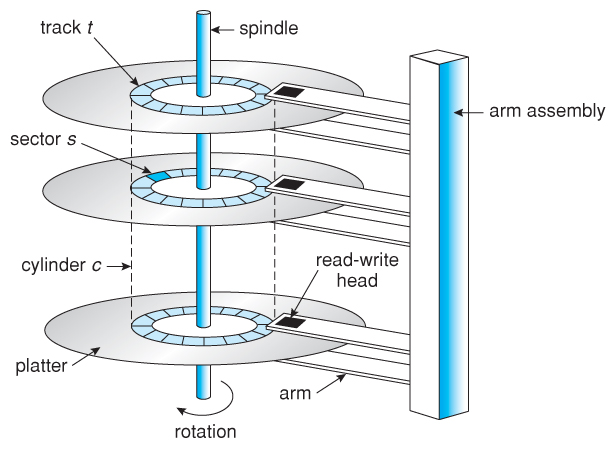
\includegraphics[width=.8\linewidth]{data-storage-architecture/arm-assembly-diagram}
	\caption{Arm Assembly Diagram}
	\label{img:arm-assembly-diagram}
\end{figure}

& Arm: Component which moves along platters to read data
	&& Head: Component on an arm which reads data

& Platter: Single double-sided physical plate in a hard drive which rotates
	&& \textbf{Track:} Circular section of data on a platter
		&&& \textbf{Cylinder:} Set of circular tracks vertically adjacent across all platters
	&& \textbf{Sector:} Pie-shaped section of a platter, from the outer edge to the middle
		&&& \textbf{Track sector:} Section of a track in a specific sector

& Read/write movements:
	&& Seek time: High-cost time required to position an arm on a disk
	&& Rotational delay: High-cost time required to rotate a platter to a position
	&& Transfer time: Low-cost time to read data from the disk with the head

& I/O operations are high-cost because they need mechanical components
	&& Read: Transfer of data from disk to main memory
	&& Write: Transfer of data from main memory to disk

\end{easylist}
\subsection{Data Pages and Frames}
	\label{subsec:data-pages-and-frames}
\begin{easylist}
	
& \textbf{Page:} Fixed-size block of data
	&& Files are stored as a collection of pages
	&& On physical disk:
		&&& Consists of a contiguous set of sectors on a single track
		&&& Smallest possible unit of data retrieval
		&&& Location impacts performance
		&&& Page ID is uniquely identified by $(b, t, c, d)$: Block $b$ of track $t$ of cylinder $c$ of disk $d$
	
	&& \textbf{Next page concept:} Sequential ordering of pages on the disk to minimize access time
		&&& Process:
			&&&& Next page on the same track
			&&&& Next page on the same cylinder
			&&&& Next page on the adjacent cylinder 
		&&& Minimizes seek and rotational delay

	&& \textbf{Sequential scan:} Reading of multiple disk pages sequentially
		&&& Allows pre-fetching of several pages at a time
	&& Fragmentation: Deleted data leaves unallocated spaces of varying sizes on a disk
		&&& Means that files are not guaranteed to be stored sequentially on disk


& \textbf{Frame:} Fixed-size space for data in physical memory
	&& For any read/write operation, the target data must first be in memory (i.e. the page containing the data must be allocated in a frame)

	&& \textbf{Dirty frame:} Frame which has unsaved modifications
		&&& A bit is used to mark dirty status upon modification
	&& \textbf{Pinned frame:} Frame which is currently in use and cannot be replaced
		&&& \textbf{Pin count:} Number of currently active users of a page

\end{easylist}
\subsection{Accessing Data Pages}
	\label{subsec:accessing-data-pages}
\begin{easylist}

& \textbf{Page fault:} Operation when a page is required but not currently in memory
	&& If a page fault occurs:
		&&& A non-pinned frame is selected
		&&& If the frame is dirty, it is saved to the disk
		&&& The new frame replaces the old frame
		&&& The new frame is pinned
		&&& The lookup table is updated
		&&& The address of the new frame is returned

& Access pattern: Pattern by which data pages are requested for access
	&& \textbf{Sequential flooding:} Data page access pattern where each page request is for a new page
& Replacement policy: Strategy which determines which frames are kept in memory or removed
	&& Different policies are optimized for different access patterns
	&& Examples: First-in-first-out (FIFO), least-recently-used (LRU), most-recently-used (MRU)

\clearpage

\end{easylist}
\subsection{Storing Records on a Page: Fixed-Length}
	\label{subsec:storing-records-on-a-page-fixed-length}
\begin{easylist}

& Introduction to records and fields:
	
	&& \textbf{Field:} Section of a record; represents a single primitive datatype
		&&&& Abbreviation: $Fx$ where $x$ is the number of the given field in order
		&&&& Abbreviation of the length of a field: $Lx$ where $x$ is the number of the given field in order

	&& \textbf{Record:} Section of a file; represents a unique data entity
		&&& Base address ($B$): Beginning location of a record on its page
		&&& Length of a record equals the sum of the length of all its fields
			&&&& Calculation: $L = \sum Li$
			&&&& Location of the $i^{\textrm{th}}$ record: $B = (i-1) \times L$
		&&& \textbf{Slot:} Location of a record on a page
		&&& \textbf{Record ID (RID):} Location of a record
			&&&& Identified by (page ID, slot \#)

& \textbf{Fixed-length record format:} Data page format where all records have the same types and numbers of fields
	&& Length of records are identical
	&& Diagram: See figure~\ref{img:record-fixed}
	
	\begin{figure}[!htb]
		\centering
		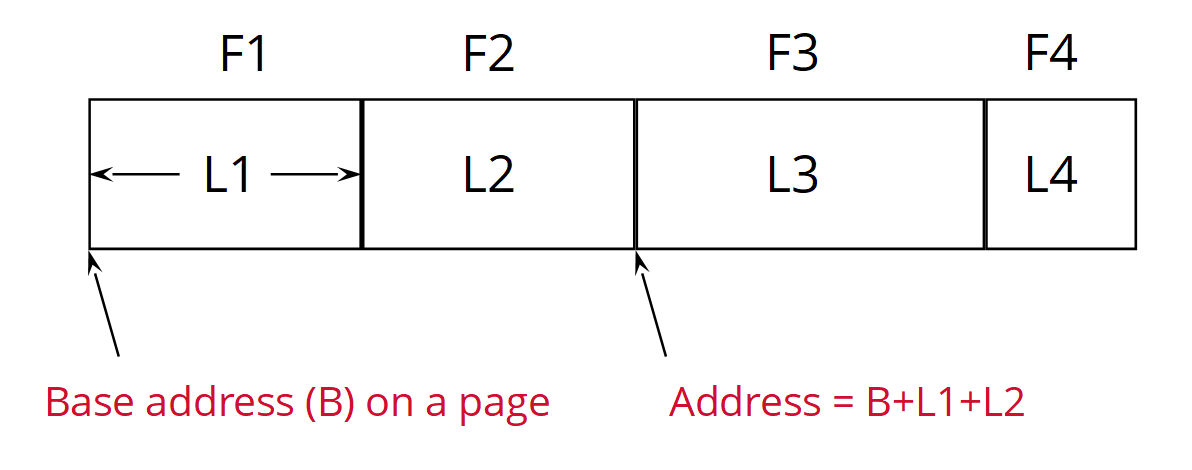
\includegraphics[width=.8\linewidth]{data-storage-architecture/record-fixed}
		\caption{Fixed-length record format}
		\label{img:record-fixed}
	\end{figure}


& \textbf{Packed page:} Fixed-length record format where free space is always organized contiguously
	&& Diagram: See figure~\ref{img:record-fixed-packed}
	
	\begin{figure}[!htb]
		\centering
		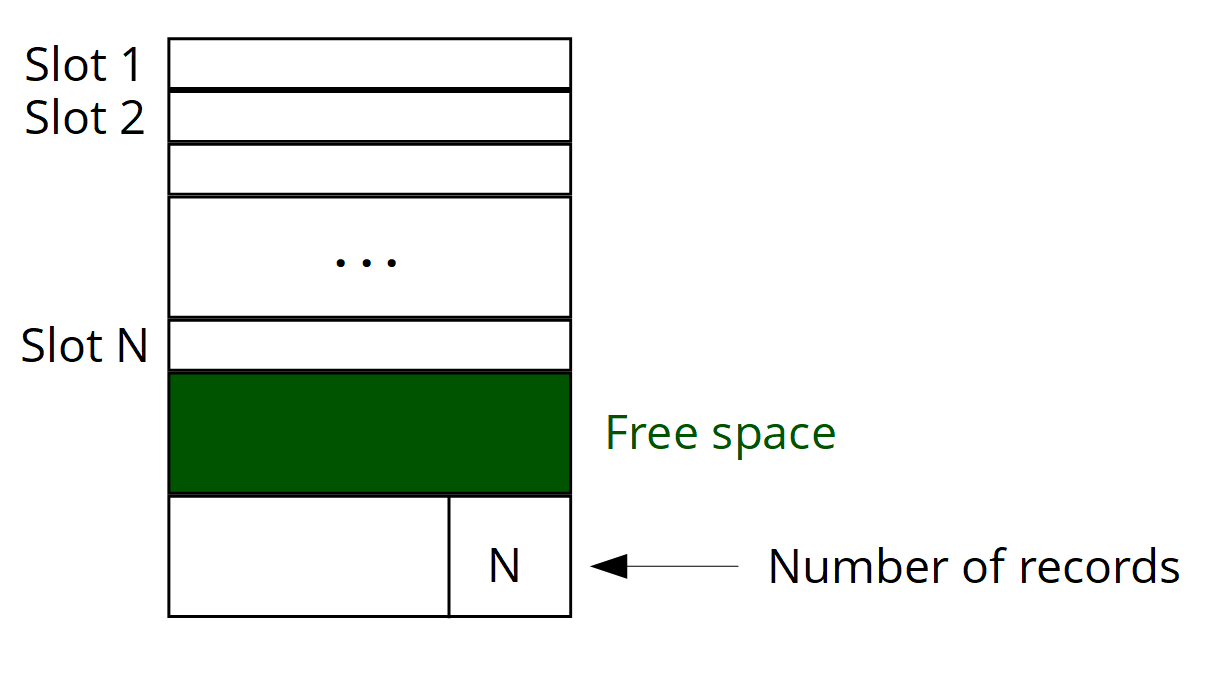
\includegraphics[width=.8\linewidth]{data-storage-architecture/record-fixed-packed}
		\caption{Packed page with fixed-length ecords}
		\label{img:record-fixed-packed}
	\end{figure}
	
	&& Contains a value with the number of currently allocated records
	&& Record addition: Allocate a slot from the start of free space
	&& Record deletion: De-allocate the slot, move the following data up to be contiguous
	&& Incurs no operation overhead as the data is in memory

& \textbf{Unpacked page:} Fixed-length record format where free space is not contiguous
	&& Diagram: See figure~\ref{img:record-fixed-unpacked}
	
	\begin{figure}[!htb]
		\centering
		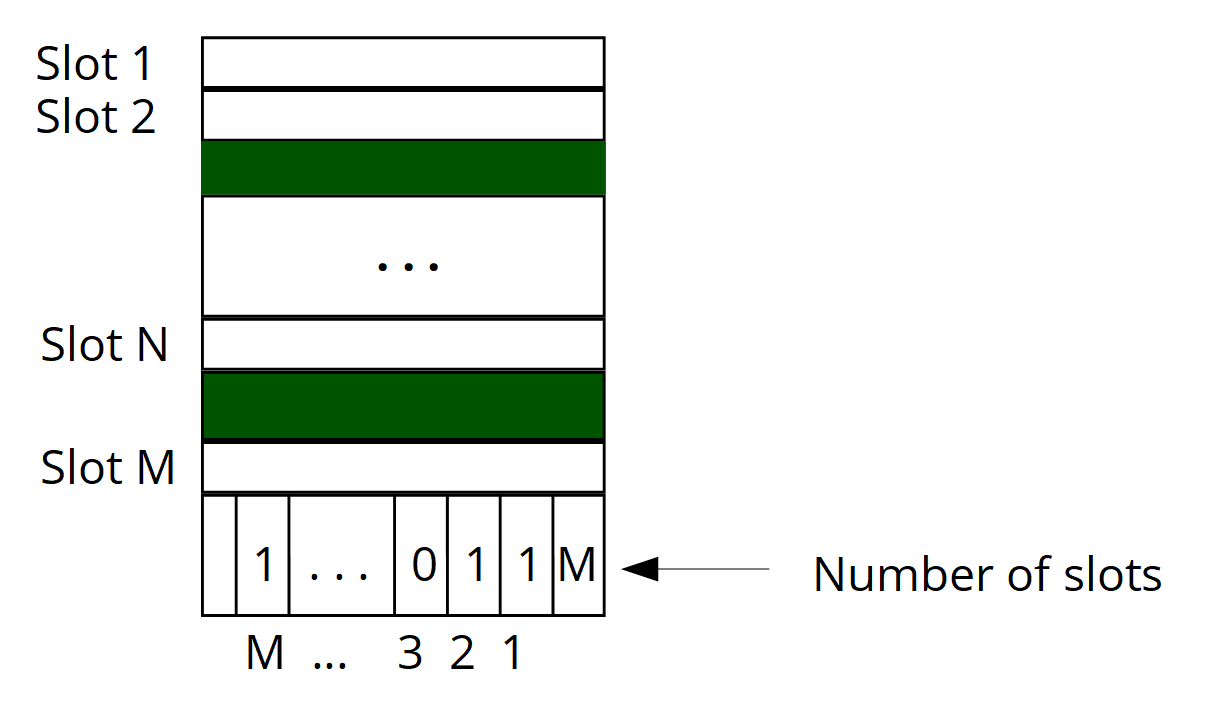
\includegraphics[width=.8\linewidth]{data-storage-architecture/record-fixed-unpacked}
		\caption{Unpacked page with fixed-length records}
		\label{img:record-fixed-unpacked}
	\end{figure}
	
	&& Contains a value with the number of currently unallocated records
	&& Free space is tracked by a bitmap at the end of the page, which represents whether a slot is allocated or free
	&& Record addition: Check the bitmap to find a free slot to allocate
	&& Record deletion: De-allocate the slot in the bitmap
	&& Incurs no operation overhead as the data is in memory

\end{easylist}
\subsection{Storing Records on a Page: Variable-Length}
	\label{subsec:storing-records-on-a-page-variable-length}
\begin{easylist}

& \textbf{Variable-length record format:} Record format where each record on a page may have differing fields
	&& Records contain a value representing the number of fields

	&& \textbf{Fixed-fields variable-length record format:} Data page format where, for all records, the number of fields cannot dynamically change (but the records may have differing fields)
		&&& Diagram: See figure~\ref{img:record-variable-fixed}
	
		\begin{figure}[!htb]
			\centering
			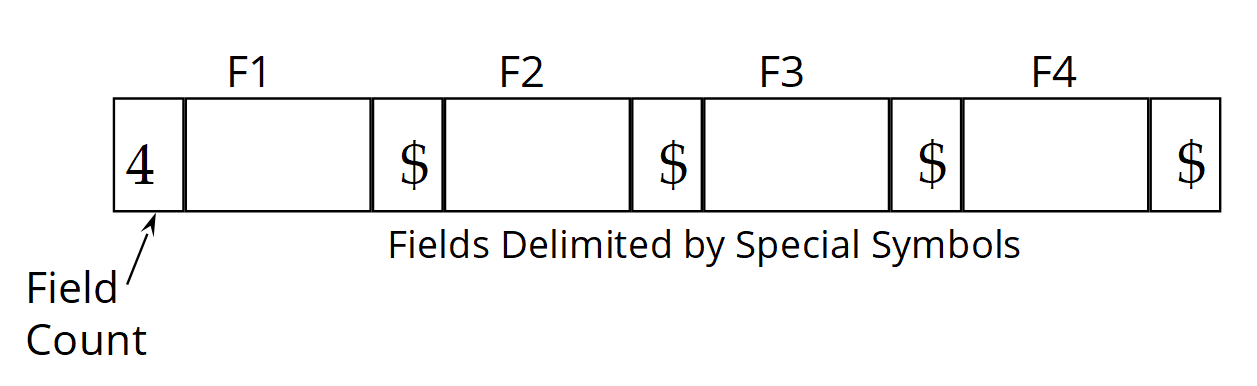
\includegraphics[width=.8\linewidth]{data-storage-architecture/record-variable-fixed}
			\caption{Variable-length records with fixed fields}
			\label{img:record-variable-fixed}
		\end{figure}
	
		&&& Fields are delimited by unique symbols
		&&& Access method: Sequential scan from beginning to end
	
	&& \textbf{Variable-fields variable-length record format:} Data page format where, for all records, the number of fields cannot dynamically change (but the records may have differing fields)
		&&& Diagram: See figure~\ref{img:record-variable-variable}
	
		\begin{figure}[!htb]
			\centering
			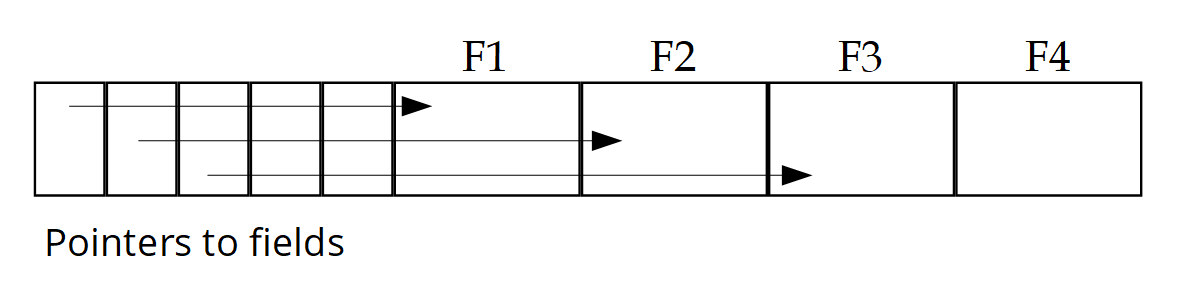
\includegraphics[width=.8\linewidth]{data-storage-architecture/record-variable-variable}
			\caption{Variable-length records with variable fields}
			\label{img:record-variable-variable}
		\end{figure}
		
		&&& Record contains a set of pointers to each field
			&&&& Incurs a space overhead
		&&& Access method: Directly from the set of pointers
		&&& Allows easy nullable storage


& Storage of variable-length records on a page:
	&& Diagram: See figure~\ref{img:record-variable-page}
	
	\begin{figure}[!htb]
		\centering
		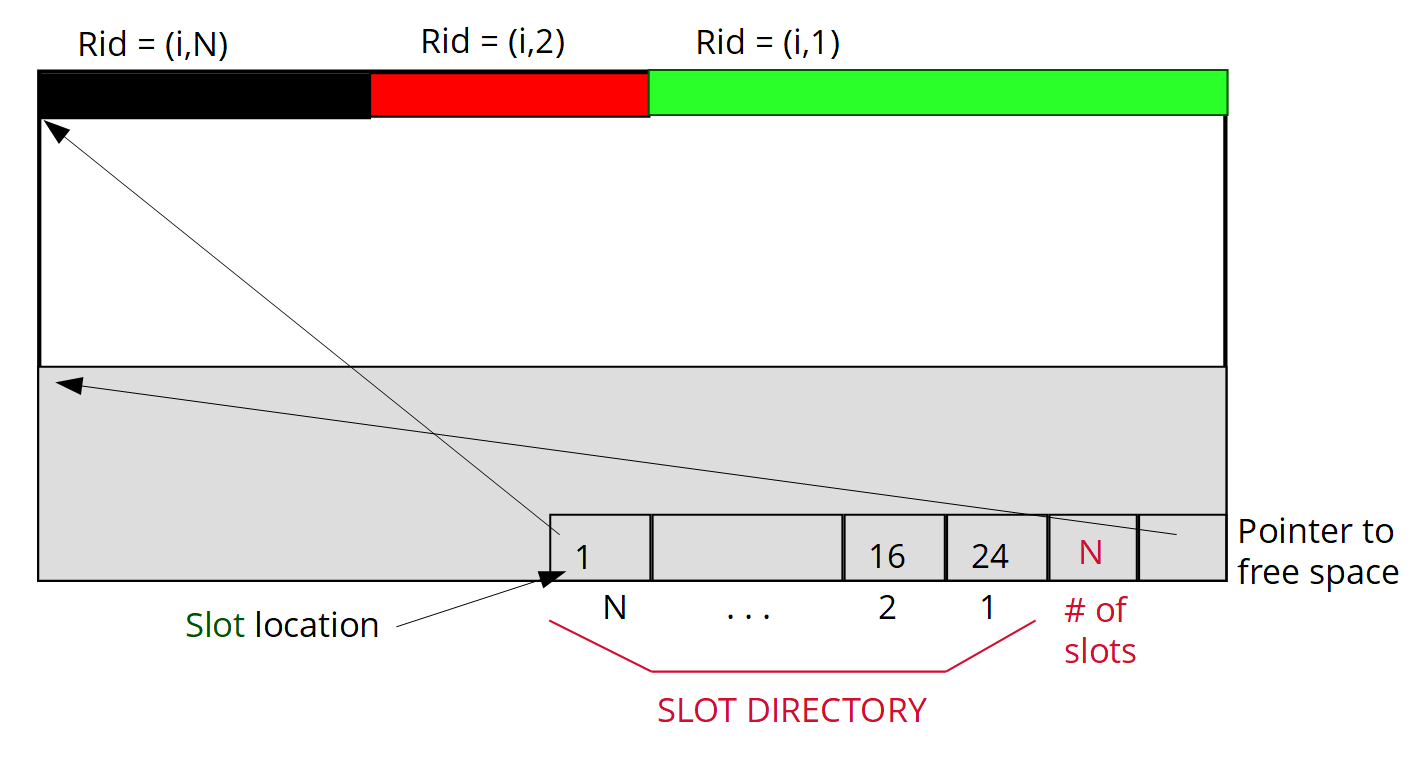
\includegraphics[width=.8\linewidth]{data-storage-architecture/record-variable-page}
		\caption{Page of variable-length records}
		\label{img:record-variable-page}
	\end{figure}
	
	&& Page contains a:
		&&& Value with the number of currently allocated slots
		&&& Pointer to first available free space
		&&& Slot directory (at the end of the page) with the starting location of each records
	&& Records are allocated by filling the next free space, and linking to it with any free slot in the directory



\end{easylist}
\clearpage














	%
% CMPT 454: Database Systems II - A Course Overview
% Section: Heap File Structure
%
% Author: Jeffrey Leung
%

\section{Heap File Structure}
	\label{sec:heap-file-structure}
\begin{easylist}

& \textbf{Logical record:} Abstract concept of data which can be inserted/deleted/modified/searched
	&& Value-based searches include:
		&&& Equality search: Search for records equal to a given value
		&&& Range search: Search for records greater/less than a given value

& \textbf{Heap files:} File organization structure where records are unordered
	&& Disk pages are allocated/deallocated dynamically as required
	&& Efficient for inserting, searching by RID, and file scanning
	&& Inefficient for searching values of the fields

& \textbf{Linked list heap file implementation:} Heap file implementation containing one linked list with full pages, and one linked list with unallocated pages
	&& Allocation process: Search through each non-full page to find one with enough space
	&& Diagram: See figure~\ref{img:heap-file-linked-list}
		
	\begin{figure}[!htb]
		\centering
		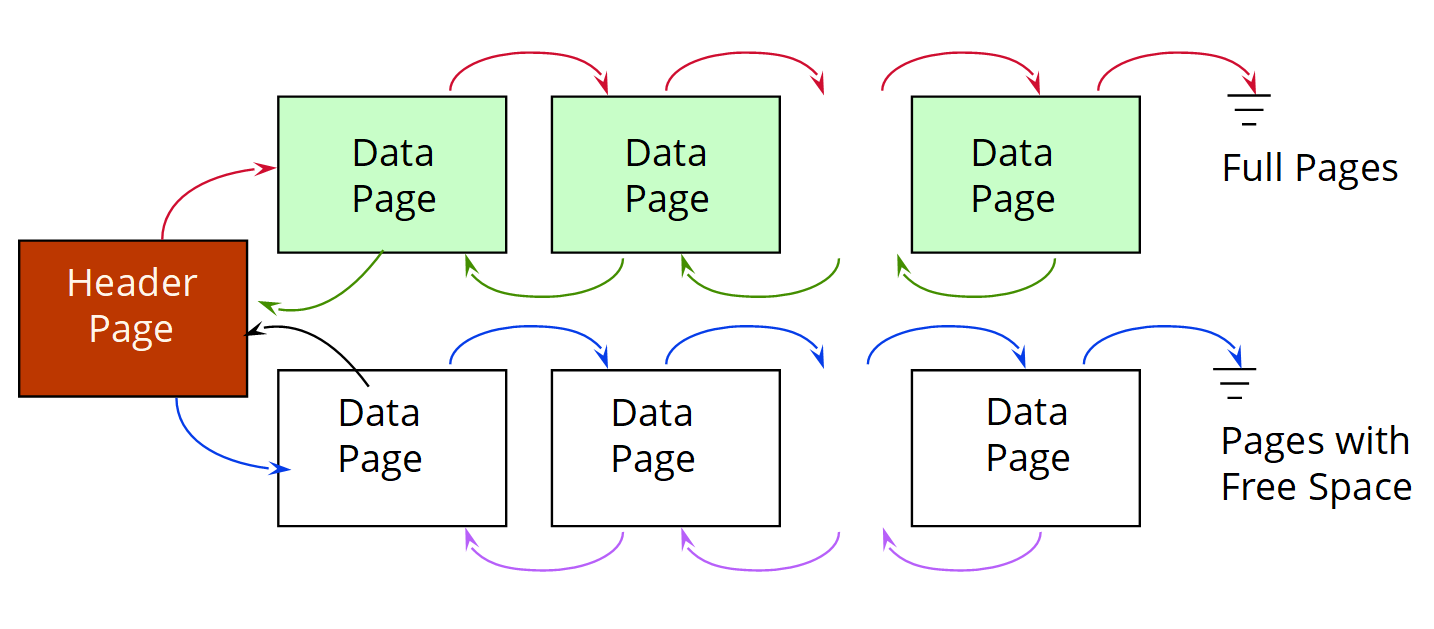
\includegraphics[width=.8\linewidth]{data-storage-architecture/heap-file-linked-list}
		\caption{Heap File: Linked List Implementation}
		\label{img:heap-file-linked-list}
	\end{figure}

& \textbf{Page directory heap file implementation:} Heap file implementation consisting of a linked list where each node contains a set of pointers to pages, and the amount of free space on the pages
	&& Allocation process: Search through nodes to find a page with enough space (reading only one page)
	&& Diagram: See figure~\ref{img:heap-file-page-directory}
		
	\begin{figure}[!htb]
		\centering
		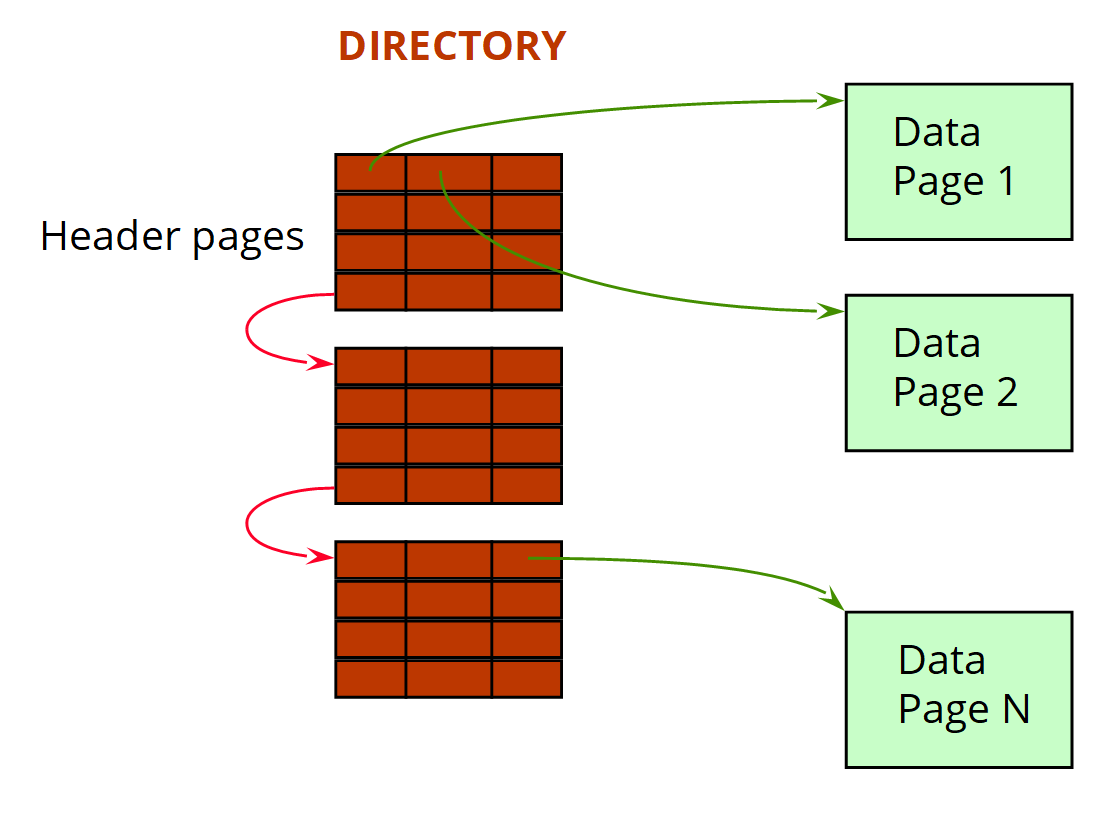
\includegraphics[width=.8\linewidth]{data-storage-architecture/heap-file-page-directory}
		\caption{Heap File: Page Directory Implementation}
		\label{img:heap-file-page-directory}
	\end{figure}

\end{easylist}
\clearpage
	%
% CMPT 454: Database Systems II - A Course Overview
% Section: Indexed File Structure
%
% Author: Jeffrey Leung
%

\section{Indexed File Structure}
	\label{sec:indexing}

\subsection{Introduction}
	\label{subsec:indexing-introduction}
\begin{easylist}

& \textbf{Indexed file structure:} File organization structure where records are organized and searchable by certain configured search keys
	&& Designed to be efficient for value-based searches

& Structure of an index:

	&& \textbf{Search key:} Field(s) on which a file/record is organized for searchability
		&&& Not guaranteed to be unique
		&&& Creating an index associates each record with a corresponding search key
		&&& \textbf{Composite search key:} Search key composed of multiple fields
			&&&& Sorting by a composite key sorts by its fields in order

	&& \textbf{Data entry:} Single search key and IDs of all records which contain/match it
		&&& Notation: Given search key value $k$, the index emits a set of data entries $k*$
		&&& Always sorted by the search key $k$
		&&& Possible formats:
			&&&& $\langle k \textrm{, data record} \rangle$
				&&&&& DB cannot have any other indices
			&&&& $\langle k \textrm{, RID} \rangle$
			&&&& $\langle k \textrm{, list of RIDs} \rangle$

\end{easylist}
\subsection{Types of Indices}
	\label{subsec:types-of-indices}
\begin{easylist}
		
& Methods of indexing:
	&& \textbf{Sorted file structure:} Indexed file structure where records are sorted by search key (generally using a tree)
		&&& Efficient for equality/range searches
		
	&& \textbf{Hashed file structure:} Indexed file structure where records are grouped in buckets by a hashed search key
		&&& Efficient for equality searches
		&&& Types: Static hashing, extendible hashing, linear hashing

& \textbf{Unique index:} Index format where the search key contains a candidate key
	&& \textbf{(Candidate) Key:} Set of fields which uniquely defines a record
	&& I.e. Searching the index using a candidate key returns either 0 or 1 result

& \textbf{Clustered index:} Index for which the data records are sorted by $k$ (in addition to the data entries sorted by $k$)
	&& Maximum of 1 clustered index per file
	&& Records are sequential on the page, though the pages may have pointers to the next page rather than be sequential
	&& Diagram: See figure~\ref{img:clustered-index}

	\begin{figure}[!htb]
		\centering
		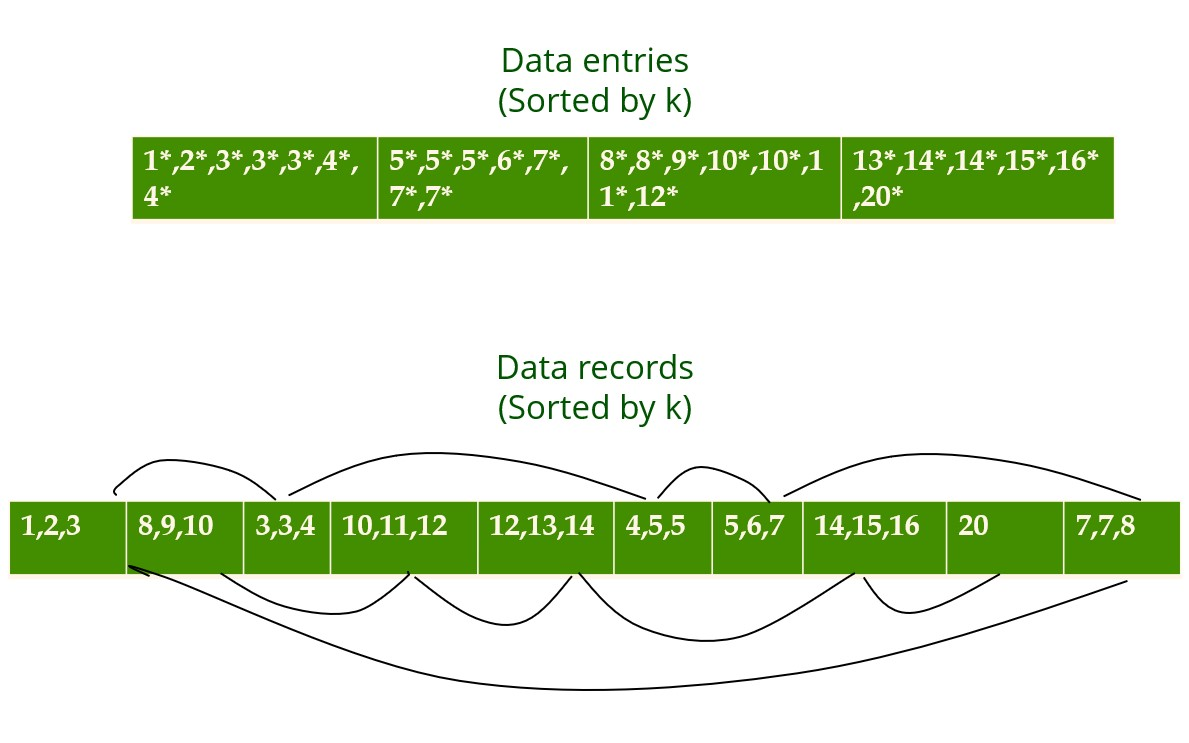
\includegraphics[width=.8\linewidth]{indexed-file-structure/clustered-index}
		\caption{A clustered index and its records}
		\label{img:clustered-index}
	\end{figure}
	
	&& \textit{Unclustered index:} Index for which the data records are not sorted by $k$
		&&& Diagram: See figure~\ref{img:unclustered-index}

		\begin{figure}[!htb]
			\centering
			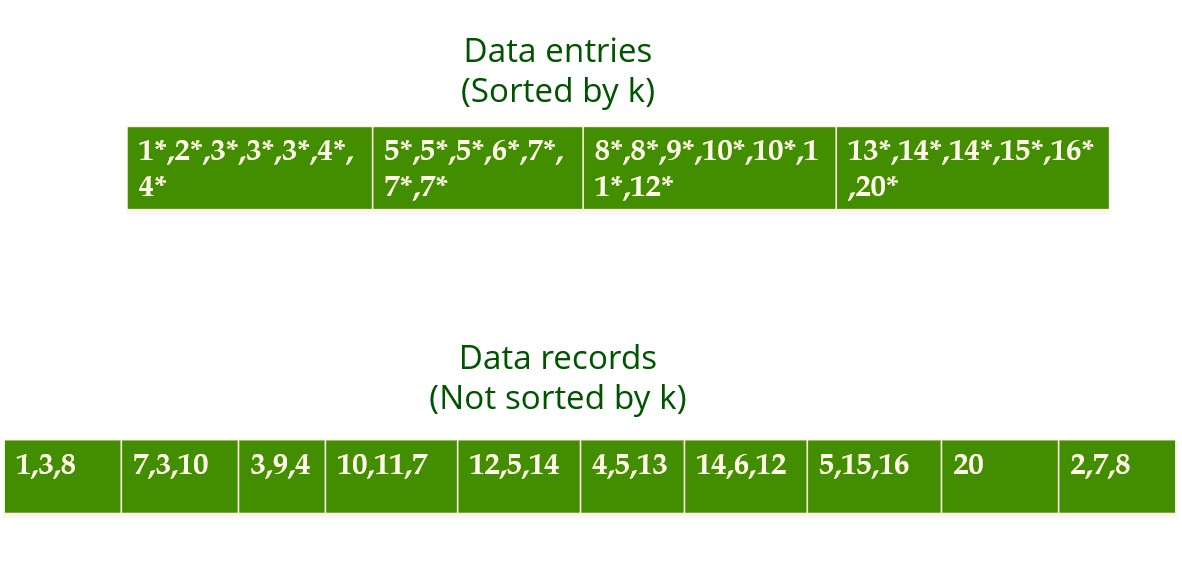
\includegraphics[width=.8\linewidth]{indexed-file-structure/unclustered-index}
			\caption{An un clustered index and its records}
			\label{img:unclustered-index}
		\end{figure}
	
	&& Data entry format $\langle k \textrm{, data record} \rangle$ is always clustered by the single index
	&& Search process for a given data range in a clustered index:
		&&& Use the data entry to find the page with the first value to read
		&&& Read through all data records in order until reaching a value greater than the end

& \textbf{Dense index:} Index where, for every search key $k$, there are one or more data entries $k*$
	&& Data entry format $\langle k \textrm{, data record} \rangle$ is always dense
	&& \textbf{Sparse index:} Index where there is at least one search key $k$ which does not map to any data entries
		&&& In a sparse index, data entries are always clustered for efficient scanning

\clearpage
\end{easylist}
\subsection{Tree-Structured Indexes}
	\label{subsec:tree-structured-indexes}
\begin{easylist}

& \textbf{Index search tree:} Search structure where index pages branch out to primary leaf pages which contain data entries
	&& Root and index pages consist of splitting keys and ordered pointers to trees containing values greater/less than the splitting keys
	&& Common components:
		&&& \textbf{Index pages:} Index search tree node which contains pivots for the search key values and pointers to index/leaf pages
			&&&& Does not directly contain data entries
			&&&& \textbf{Splitting key:} Index page value which acts as a pivot value for partitioned subtrees
			&&&& Root: Top node of an index search tree which contains a single pivot value and pointers to index pages
		&&& \textbf{Primary leaf page:} Index search tree leaf node which contains a set of data entries with pointers to data records
			&&&& Will not be deallocated even if empty

\clearpage
\end{easylist}
\subsubsection{ISAM Trees}
	\label{subsubsec:isam-trees}
\begin{easylist}

& \textbf{Indexed sequential access method (ISAM):} Index search tree where index pages are static and leaf pages contain optional overflow pages
	&& \textbf{Overflow page:} Linked list starting from a primary leaf page, which contains additional search key values
		&&& Allocated/deallocated as required; all other nodes in the tree are not affected during insert/delete operations
		&&& Can degrade performance

& Diagram: See figure~\ref{img:isam-tree}
	
\begin{figure}[!htb]
	\centering
	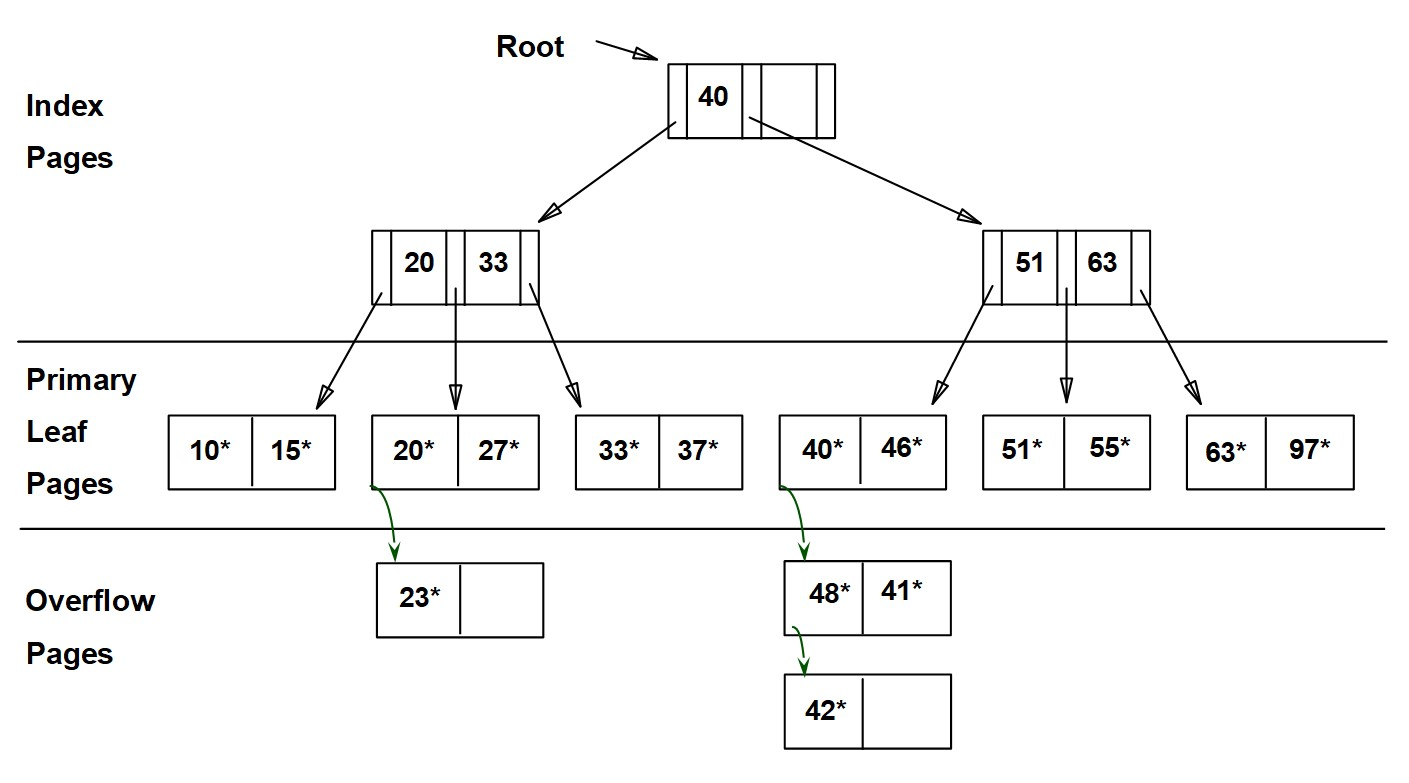
\includegraphics[width=.8\linewidth]{indexed-file-structure/isam-tree}
	\caption{An ISAM Tree}
	\label{img:isam-tree}
\end{figure}

& Search process:
	&& Follow the search from the root through the index pages to the matching primary leaf page
	&& Search the leaf page
	&& Search any linked overflow pages until a result is found
& Rebalanced during system maintenance

\clearpage
\end{easylist}
\subsubsection{B+ Trees}
	\label{subsubsec:b+-trees}
\begin{easylist}

& \textbf{B+ tree:} Index search tree which dynamically rebalances nodes and children during operation

& Diagram: See figure~\ref{img:bplus-tree}
	
\begin{figure}[!htb]
	\centering
	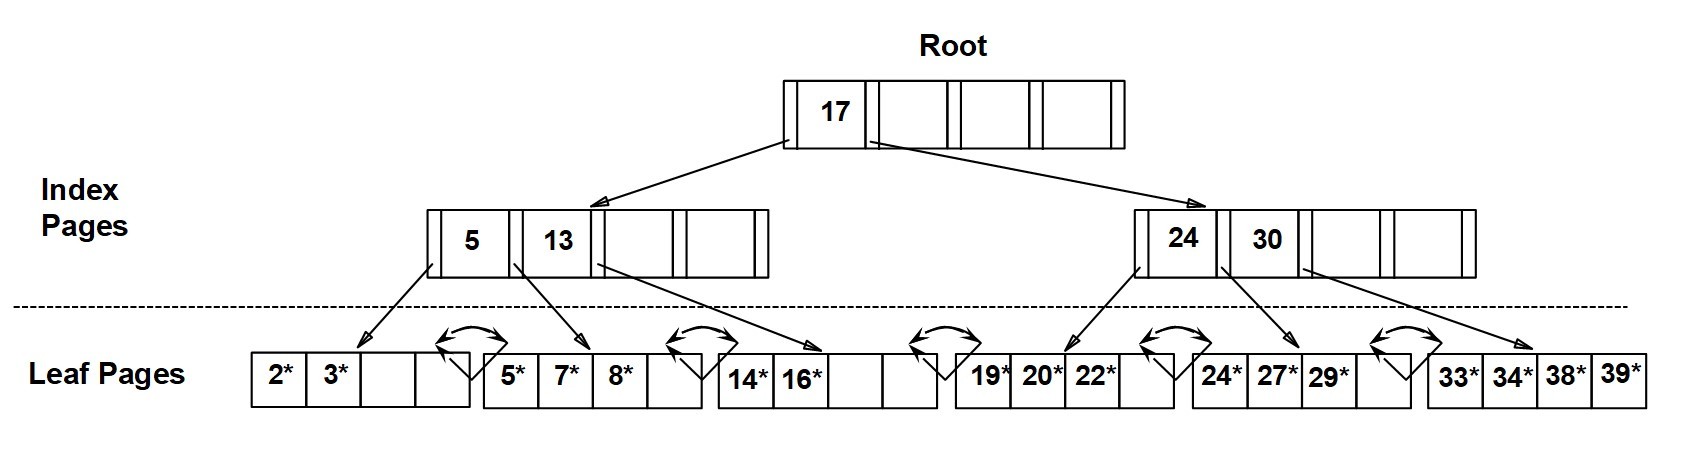
\includegraphics[width=.8\linewidth]{indexed-file-structure/bplus-tree}
	\caption{A B+ Tree}
	\label{img:bplus-tree}
\end{figure}
	
& \textbf{Order:} Minimum and maximum splitting key capacity of a B+ tree (which can differ for index and leaf nodes)
	&& Denoted by $d$
	&& Each B+ tree node must have between $d$ and $2d$ search keys (inclusive), except for the root (minimum 1)
	&& \textit{Fanout:} Branching factor of a B+ tree
		&&& Denoted by $F$
		&&& Fanout of root: $2$ to $2d+1$
		&&& Fanout of index nodes: $d+1$ to $2d+1$
		&&& Fanout of leaf nodes: $d$ to $2d$

& Ensures insert/delete/search operations are $\log_{F} N$ where $N = $ number of leaf nodes
	
& Operations:
	&& \textbf{Copying up:} B+ tree operation where a search key in a leaf is copied to the parent index node
		&&& Used when splitting a leaf in two
					
	&& \textbf{Pushing up:} B+ tree operation where a splitting key in an index node is moved to the parent index node, and removed from the original
		&&& Used when splitting an index node in two
		
	&& Insertion into a full leaf node:
		&&& Split leaf $L$ into two nodes, $L$ and $L2$
		&&& Redistribute entries evenly
		&&& Copy up the middle key to the parent to create a new partition
		&&& Link $L2$ to the parent
		&&& If the parent index node is not being split, the process is repeated recursively but with pushing-up instead of copying-up
			
	&& Deletion:
		&&& Search for and remove the entry
		&&& If the leaf node which contained the entry has only $d-1$ entries remaining:
			&&&& If the sibling node has more than $d-1$ entries, then re-balance entries with the sibling so both have at least $d-1$ entries
			&&&& Else, merge the node and its sibling (with $d$ entries) to create a node of $2d-1$ entries
				&&&&& Delete the key pointing to the deleted leaf node
				&&&&& Propagate merge upwards recursively
		
	&& \textbf{Bulk loading:} Initialization of a B+ tree with a number of records, which avoids constant rebalancing through standard insertion
		&&& Process:
			&&&& Sort data entries by search key
			&&&& Allocate data entries on the disk
			&&&& Create parent nodes for data entry leaf pages from left to right
			&&&& If the parent of the current index node has more slots available, split index nodes into siblings
			&&&& If the parent of the current index node has no slots available, split the parent node

\clearpage
\end{easylist}
\subsection{Hash-Based Indices}
	\label{subsec:hash-based-indices}
\begin{easylist}

& \textbf{Hash-based index:} Search structure where primary pages, each identified by a hashed search key, point to data entry pages
	&& Optimized for equality search; does not support range search
	&& Vulnerable to skewed hash distributions

& Common components:
	&& Hash function: Function which hashes a search key to a value
		&&& Denoted by $h(k)$ for a given data entry with search key $k$
		&&& Bucket to store the entry is chosen from $N$ buckets by calculating $h(k) \textrm{ mod } N$
	&& \textbf{Primary (bucket) page:} Hash-based index page identified by a hashed search key and containing/linking to a bucket with data entries
		&&& Always allocated sequentially for speed of access
	&& \textbf{Directory:} Collection of primary pages
		&&& Not in all types of hash indices
	&& \textbf{Overflow page:} Hash index page containing data entries, linked to from a primary page
		&&& Not in all types of hash indices
		&&& Allocated and de-allocated as required

\clearpage
\end{easylist}
\subsubsection{Static Hashing}
	\label{subsubsec:static-hashing}
\begin{easylist}

& \textbf{Static hashing:} Hash-based index method where the primary pages are never modified or deallocated
	&& Uses overflow pages to hold additional data entries
		&&& May create overflow chains when there are too many records, or hashes skew towards several values
		
& Diagram: See figure~\ref{img:static-hashing}
\begin{figure}[!htb]
	\centering
	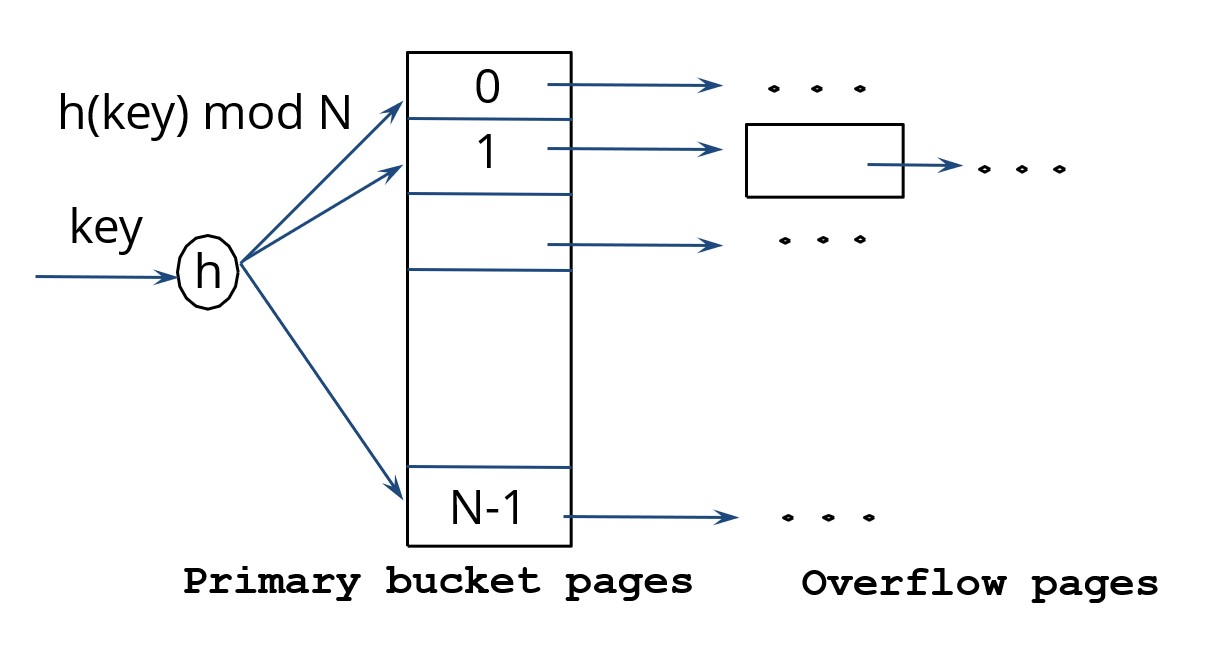
\includegraphics[width=.8\linewidth]{indexed-file-structure/static-hashing}
	\caption{A Static Hash Index}
	\label{img:static-hashing}
\end{figure}

\clearpage
\end{easylist}
\subsubsection{Extendible Hashing}
	\label{subsubsec:extendible-hashing}
\begin{easylist}

& \textbf{Extendible hashing:} Hash-based index method which splits overflowing buckets and dynamically increases the directory
	&& Does not use overflow pages
	&& When a bucket overflows, its contents are split into a new bucket which is added to the directory
	&& Requires accessing a directory page to look up an entry page
	&& Bucket access is approximately 1.2 page accesses amortized (due to overflows)

& \textbf{Global depth:} Value on an extendible hashing directory which tracks the number of bits in the current directory size
& \textbf{Local depth:} Value on an extendible hashing bucket which (approximately) tracks the number of buckets matching the same hash
	&& If local depth is less than global depth, then the bucket can be split without increasing directory size
	&& If local depth equals the global depth, then splitting the bucket will require doubling the directory
	
& Diagram: See figure~\ref{img:extendible-hashing}

\begin{figure}[!htb]
	\centering
	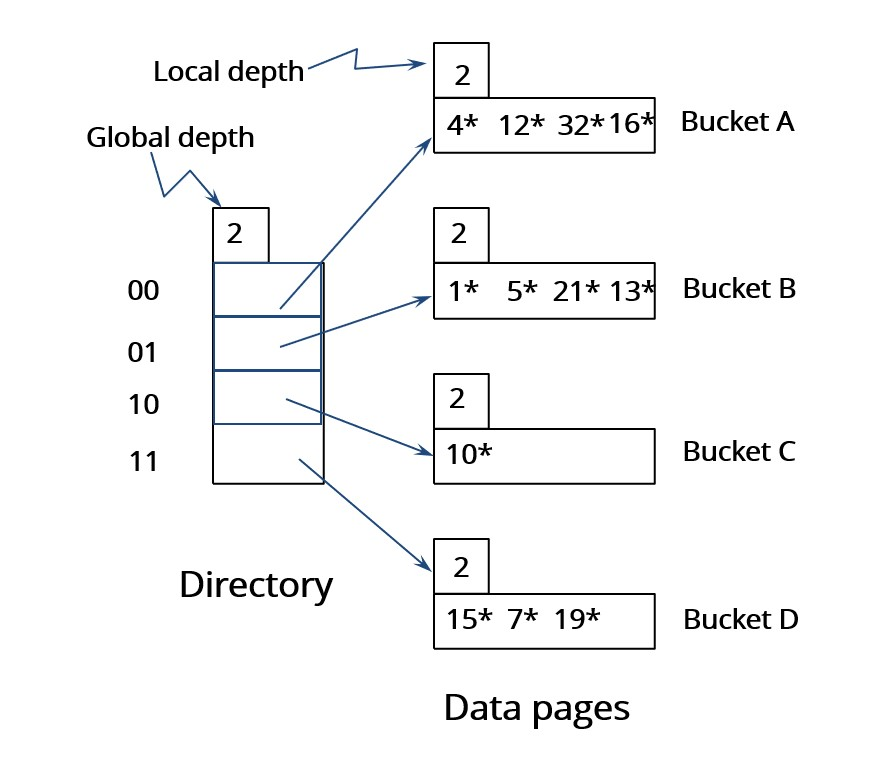
\includegraphics[width=.8\linewidth]{indexed-file-structure/extendible-hashing}
	\caption{An Extendible Hash Index}
	\label{img:extendible-hashing}
\end{figure}

\clearpage
& Operations:

	&& Insertion:
		&&& When a bucket overflows, split its contents into a new bucket of the same hash
		&&& Increment the local depth of both buckets
		&&& If the directory has no space for a new bucket of the same hash (i.e. the global depth is less than the new local depth), the directory is increased to accommodate hashing the new bucket:
			&&&& Double the directory (adding a new leftmost bit to the directory index)
			&&&& Increment the global depth
			&&&& Point the newly created directory indices to the existing buckets with the same hash values
		&&& Link the new duplicate hash value in the directory to the new bucket
		
		&&& Diagram: See figure~\ref{img:extendible-hashing-splitting}
		\begin{figure}[!htb]
			\centering
			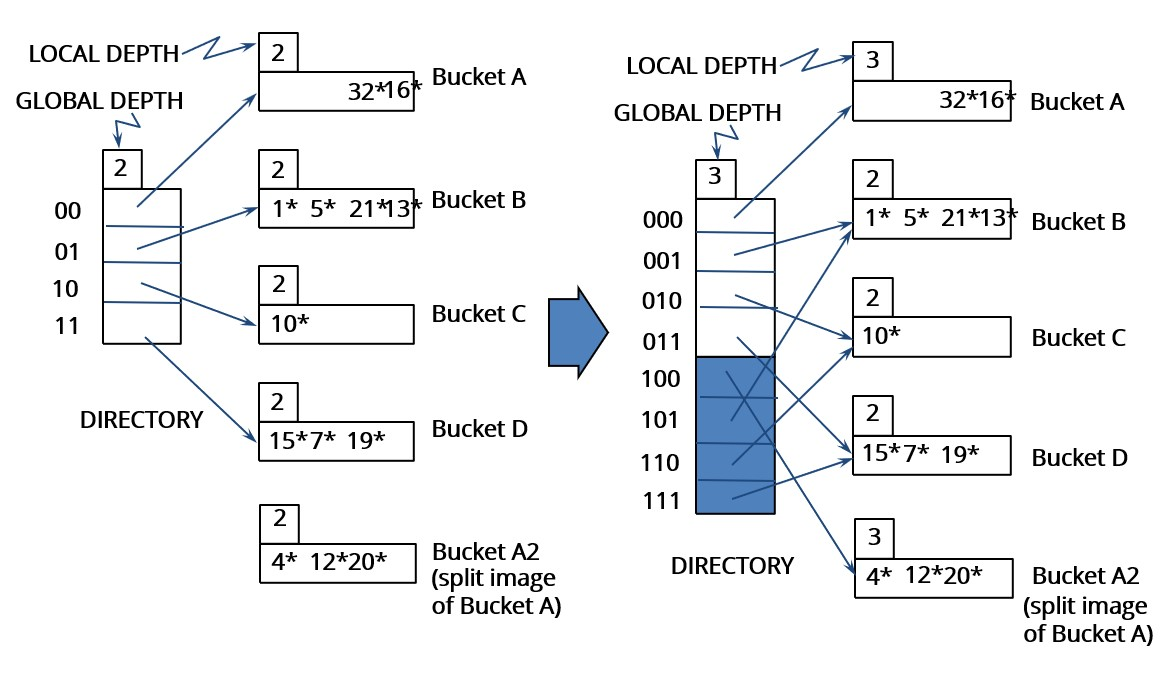
\includegraphics[width=.8\linewidth]{indexed-file-structure/extendible-hashing-splitting}
			\caption{Splitting an Extendible Hash Bucket}
			\label{img:extendible-hashing-splitting}
		\end{figure}
		
	&& Deletion:
		&&& Remove the data entry from the corresponding bucket
		&&& If the bucket has no more entries, deallocate it and point the key in the directory to the matching bucket
		&&& If half or more of the buckets of all hashes are empty/deallocated, the directory can be halved

\clearpage
\end{easylist}
\subsubsection{Linear Hashing}
	\label{subsubsec:linear-hashing}
\begin{easylist}

& \textbf{Linear hashing:} Hash-based index method which uses overflow pages, splits buckets using a round-robin strategy, and dynamically doubles the buckets
	&& Has no directory; does not require directory page lookup before accessing an entry page
	&& Splits a bucket into two (chosen by round-robin strategy) whenever any overflow page is created
		&&& Every bucket is kept split evenly, rather than focusing on splitting heavy-use buckets
	&& Bucket access is approximately 1.2 page accesses amortized (due to overflows)
	
& Components:

	&& \textbf{Overflow page (linear hashing):} Data bucket which holds additional data entries matching the index, which have not yet been split into new buckets
	
	&& Uses two hash algorithms at any given time; when the buckets are doubled, the old one is discarded and a new hash algorithm is added

	&& \textbf{Level:} Index of the hash algorithms currently being used, and the number of times the buckets have been doubled
		&&& Begins at 0; increments without limit
		&&& Hash algorithm of a certain level $x$ is denoted by $h_x$

	&& \textbf{Next:} Beginning index of buckets in a linear hashing index which have not yet been split
		&&& Begins at 0; increments when a bucket is split; reset to 0 after splitting all buckets once
		&&& All buckets before \textrm{next} have been split in the current round-robin implementation
			&&&& All buckets after or including \textrm{next} have not yet been split in the current round-robin implementation

		
& Diagram: See figure~\ref{img:linear-hashing}
\begin{figure}[!htb]
	\centering
	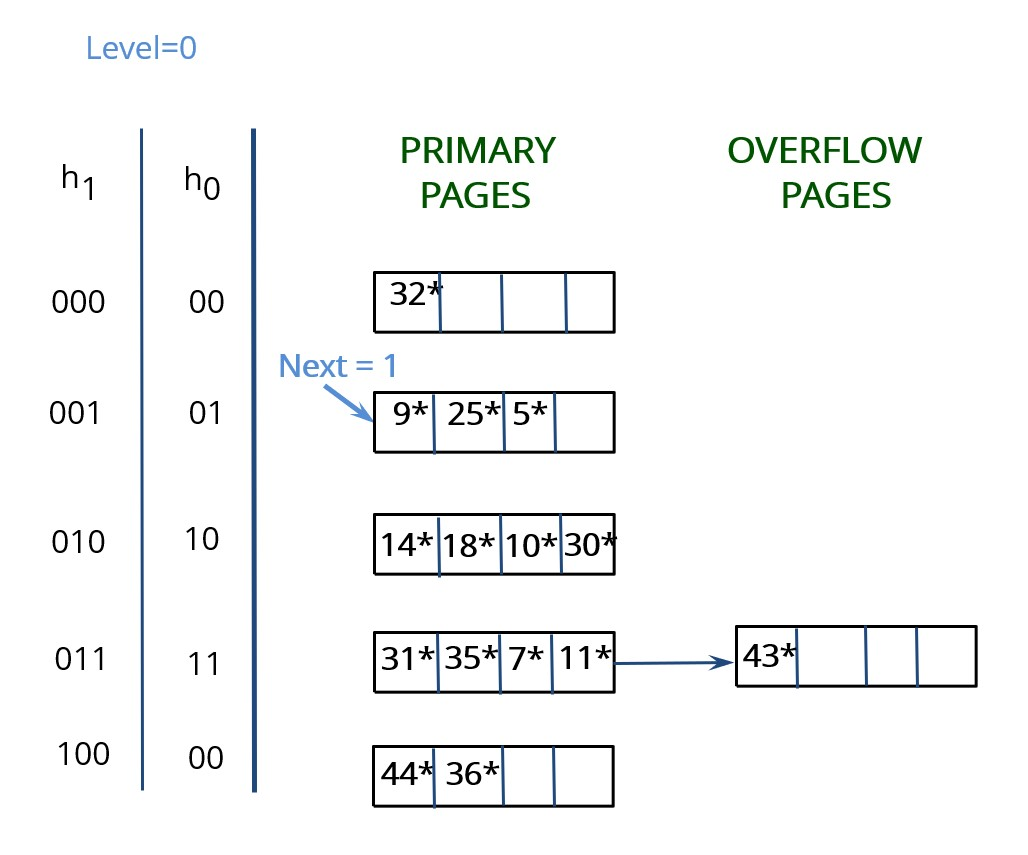
\includegraphics[width=.8\linewidth]{indexed-file-structure/linear-hashing}
	\caption{A Linear Hash Index}
	\label{img:linear-hashing}
\end{figure}
		
& Operations:	
			
	&& Search:
		&&& Use $h_\textrm{level}$ to find the index of the bucket where the value belongs
			&&&& If the index is less than \textrm{next}, the search key belongs in the index found by $h_\textrm{level+1}$ (as the bucket has been split)
			&&&& If the index is greater than or equal to \textrm{next}, the search key belongs in this (as the bucket has not yet been split)
		&&& Search the selected bucket and any linked overflow pages
	
	&& Insertion:
		&&& Apply the search process above to find the bucket to insert the data entry
		&&& Add the value to the bucket, creating an overflow page if necessary
		
		&&& If an overflow page is created:
			&&&& Split the bucket at index \textrm{next}
			&&&& Index the new bucket at the bottom of the others
			&&&& Use $h_\textrm{level+1}$ to redistribute the values between the old and new buckets
			&&&& Increment \textrm{next}
		
		&&& If \textrm{next} has looped through all buckets once (not including the newly split buckets):
			&&&& Discard hash algorithm $h_\textrm{level}$
			&&&& Increment \textrm{level}
			&&&& Create a new hash algorithm $h_\textrm{level+1}$
			&&&& Reset \textrm{next} to 0

\end{easylist}
\clearpage








































	%
% CMPT 454: Database Systems II - A Course Overview
% Section: External Sorting
%
% Author: Jeffrey Leung
%

\section{External Sorting}
	\label{sec:external-sorting}
\begin{easylist}

& Sorting is essential for:
	&& Outputting data in sorted order
	&& Removing duplicates
	&& Preparing data for B+ tree insertion

& B+ tree: If the data to be retrieved is clustered, then it is efficient to retrieve as sorted

& Evaluation strategy is chosen before query execution, for optimized performance

& \textbf{External sort:} Sorting algorithm which operates on primitive data pages but is not executed by the database
	&& \textbf{Run:} Sorted subfile used during a larger sort strategy
	&& \textbf{Input buffer:} Memory slot which holds data to be processed
	&& \textbf{Output buffer:} Memory slot which holds data to be written to the disk

\end{easylist}
\subsection{Merge Sort}
	\label{subsec:merge-sort}
\begin{easylist}

& Merge sort: External sorting algorithm
	&& Process:
		&&& On the first pass:
			&&&& Read pages (up to the number of buffers)
			&&&& Sort each page individually
			&&&& Write pages back to disk
			
		&&& On subsequent passes:
			&&&& Reserve a single buffer for output
			&&&& Merge two `runs' into a single run, in the output buffer
				&&&&& Given $B$ available buffers, $B-1$ runs can be merged in a single pass
			&&&& Write the output buffer back to disk
			&&&& Repeat
		&&& Diagram: See figure~\ref{img:merge-sort}

		\begin{figure}[!htb]
			\centering
			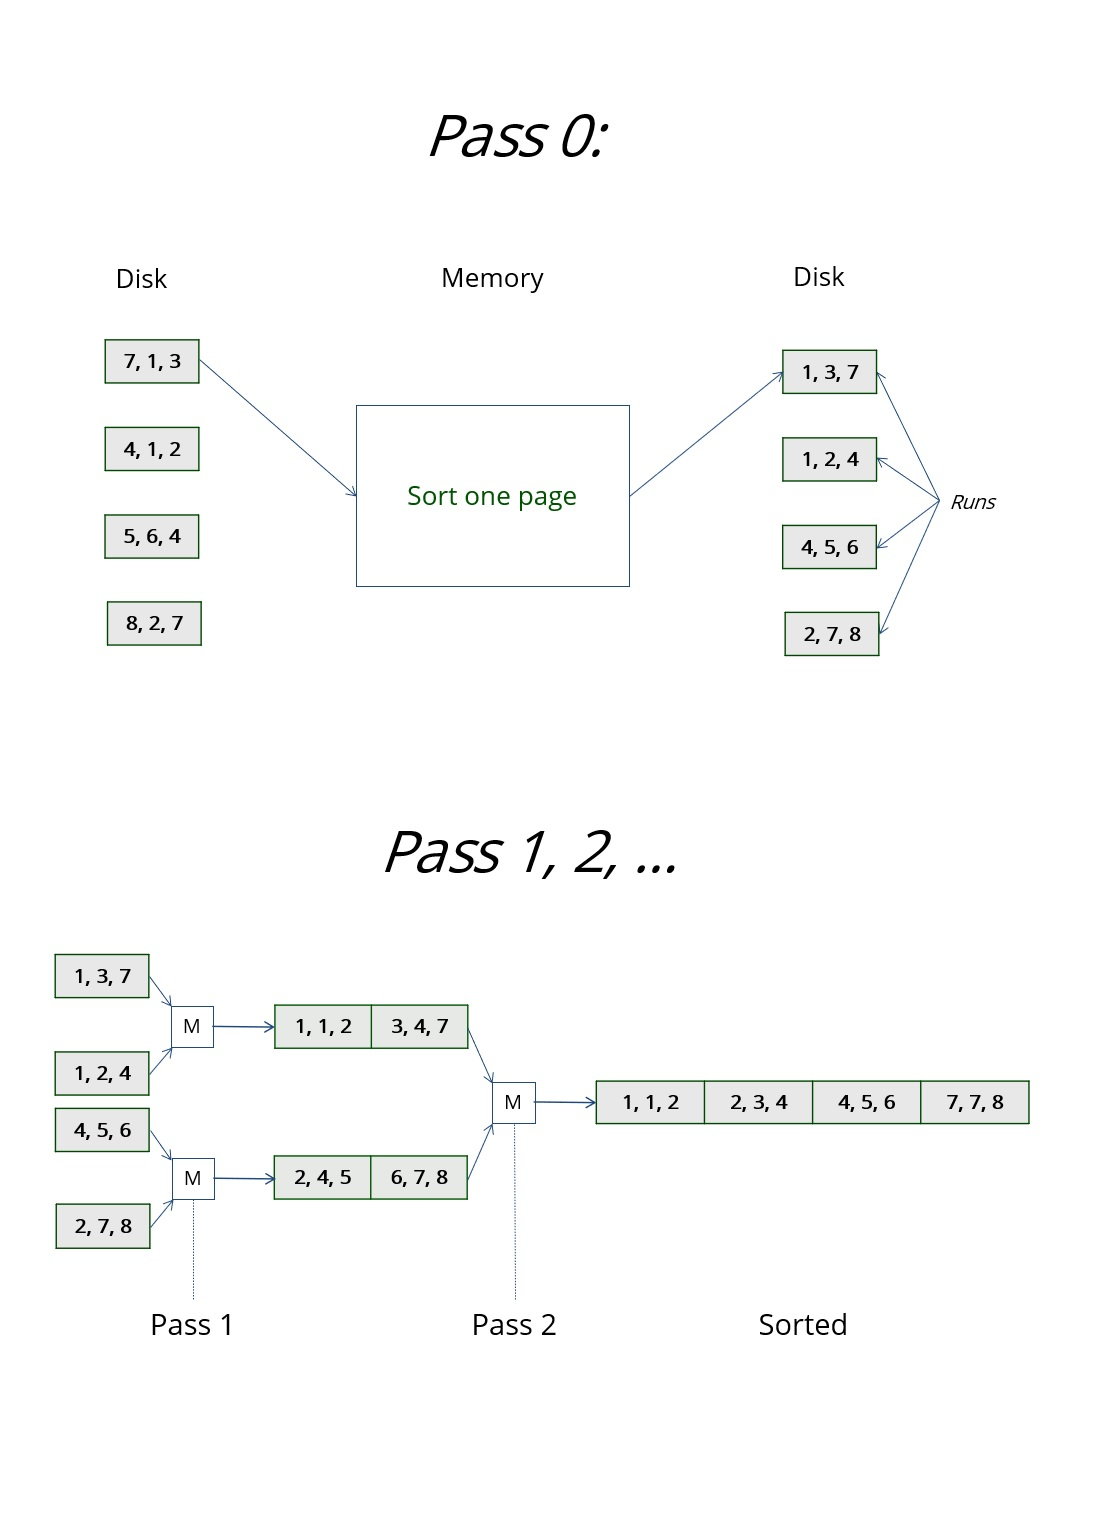
\includegraphics[width=.8\linewidth]{external-sorting/merge-sort}
			\caption{Diagram of the First and Subsequent Passes of a Merge Sort}
			\label{img:merge-sort}
		\end{figure}

& Page I/O (given $n$ data pages to sort):
	&& $n$ for the first pass
	&& $2n$ for each subsequent pass (as each processed value is read once and written once)
	
& Buffer management:
	&& Given $n$ available buffers:
		&&& One buffer is used as an sorted output buffer (written to disk whenever full and emptied)
		&&& $n-1$ buffers are used to track one run each, from which data is fed into the output buffer
	&& Merge as many buffers as possible during each pass, to minimize time

\clearpage
\end{easylist}
\subsection{Replacement Sort}
	\label{subsec:replacement-sort}
\begin{easylist}
	
& \textbf{Replacement sort:} External sorting algorithm where a sorted run is continuously built from a current working set of available data
	&& Consists of one input buffer, one `current set' of sortable data, and one output buffer
	&& Process:
		&&& Whenever the input buffer is empty, fill it with a new page from the disk
		&&& Whenever the current set has an empty slot, fill it with data from the input buffer
		&&& From the current set, take the value which meets the following conditions and add it to the output buffer:
			&&&& The minimum possible value in the set, and
			&&&& Equal or greater than the maximum value in the output buffer
		&&& Whenever the output buffer is full, write it to disk and empty it
		&&& Repeat until all data has been read from the disk once (completing one round)
		&&& Repeat rounds until the current set is empty at the end of the round

& Diagram: See figure~\ref{img:replacement-sort}

\begin{figure}[!htb]
	\centering
	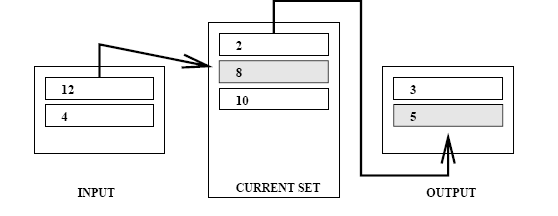
\includegraphics[width=.8\linewidth]{external-sorting/replacement-sort}
	\caption{Diagram of the Replacement Sort Data Structure}
	\label{img:replacement-sort}
\end{figure}

\end{easylist}
\clearpage
	%
% CMPT 454: Database Systems II - A Course Overview
% Section: Query Optimization
%
% Author: Jeffrey Leung
%

\section{Query Optimization}
	\label{sec:query-optimization}
\begin{easylist}

& Notation: Given a schema $R$:
	&& The size in pages is denoted as $|R|$
	&& The number of records per page is denoted as $p_R$
	&& The size of the buffer is $B$

& Clustered indices are only applicable for terms which form a prefix of the search key
	&& E.g. The index $<A, B, C>$ can be used for the search key $A = 1, B = 3$

\clearpage
\end{easylist}
\subsection{Optimizing Equality Joins}
	\label{subsec:optimizing-equality-joins}
\begin{easylist}

& \textbf{Join:} Database operation where a single set of rows are returned, created from two relations

& E.g. \textrm{SELECT * FROM Sailors S, Reserves R WHERE R.id = S.id}
	
& \textbf{Simple Nested Loops (SNL) join:} Equality join implementation where nested loops compare equality values using 1-page buffers
	&& Consists of multiple nested loops, each of which loops through a table
		&&& \textbf{Outer table:} Table in an SNL join which is scanned outside the other nested loop(s)
		&&& \textbf{Inner table:} table in an SNL join which is scanned inside the other nested loop(s)
	&& Runtime:
		\begin{align*}
			|Outer| + |Outer| \cdot |Inner|
		\end{align*}
		&&& $|Outer|$ is the cost of loading each value from the outer table into memory
		&&& $|Outer| * |Inner|$ is the cost of loading each value from the inner table into memory, and comparing with an outer table value
		&&& To optimize, smaller tables should be implemented as the outer
			
& \textbf{Block Nested Loops (BNL) join:} Equality join implementation where nested loops compare equality values using multi-page buffers
	&& \textbf{Block:} Fixed-size set of pages representing the size of a buffer
	&& Runtime:
		\begin{align*}
			|Outer| + |Outer\ Blocks| \cdot |Inner| \\
			= |Outer| + \left\lceil \frac{|Outer|}{B-2} \right\rceil \cdot |Inner|
		\end{align*}
		&&& Two buffer pages are used; one as the output buffer and one as the input buffer for the inner table
		&&& To optimize, smaller tables should be implemented as the outer

& \textbf{Index Nested Loops (INL) join:} Equality join implementation where nested loops compare equality values, and inner loops use an index to search matching values from the outer loop
	&& Runtime:
		\begin{align*}
			|Outer| + |Outer| \cdot p_{outer} \cdot \textrm{probing costs}
		\end{align*}
		&&& $|Outer| \cdot p_{outer}$ represents the number of records in table $R$
		&&& \textbf{Probing cost:} I/O cost to search for an entry and record using an index
			&&&& Probing cost of data entries in a hash index: 1.2
			&&&& Probing cost of data entries in a B+ tree: 3-4
			&&&& Probing cost of data records when the search key is a candidate key: 1
			&&&& Probing cost of data records when the search key is not a candidate key, in a clustered index: 1
			&&&& Probing cost of data records when the search key is not a candidate key, in an unclustered index: $\frac{\textrm{records in inner}}{\textrm{records in outer}}$
				
	&& Equality with multiple attributes: Index must apply to one or more of the attributes
	&& Inequality: Index must be clustered B+ tree

& \textbf{Sort-merge-join (SMJ):} Equality join implementation where tables are sorted externally, written back to the disk, merged by equality, then sent to output
	&& Runtime:
		&&& Sorting:
		\begin{align*}
			  2 \cdot |T_1| \cdot (\left\lceil \log_{B-1} (\frac{|T_1|}{B}) \right\rceil + 1) \\
			+ 2 \cdot |T_2| \cdot (\left\lceil \log_{B-1} (\frac{|T_2|}{B}) \right\rceil + 1)
		\end{align*}
		where $T_1$, $T_2$ are tables and $B$ is the buffer size
		&&& Merging:
		\begin{align*}
			|T_1| + |T_2|
		\end{align*}
		&&& Optimization 1: Find the tables which have the fewest maximum count of any repeating value, then use those those tables as the outer loop (to fit as much outer loop data as possible into the input buffer)
		&&& Optimization 2: Join the runs of the sorted tables after only the first pass of the external sort
			&&&& When joining, each run is allocated a single buffer
			&&&& Only possible if $B \geq \sqrt{\textrm{max} \{ |T_1|, |T_2| \} }$
			&&&& Runtime:
			\end{easylist}
			\begin{align*}
				& \textrm{(Cost of pass 0)} + \textrm{(Merging all runs)} \\
				& = 2 (|R|+|S|) + (|R|+|S|) \\
				& = 3 (|R|+|S|)
			\end{align*}
			\begin{easylist}
				
	&& Equality with multiple attributes: Sort based on all joined attributes
	&& Inequality: Not applicable
			

& \textbf{In-memory probing by hash table:} CPU runtime optimization which hashes database table pages into buckets
	&& Reduces excess page retrieval and optimizes access speed to specific pages

& \textbf{Hash-join (HJ):} Equality join implementation where tables are partitioned into hash buckets, then the values in each hash bucket is joined with the matching values in the hash bucket from the other table
	&& Hash bucket notation:
		&&& $T_i$ represents the contents of hash bucket $i$ created by partitioning $T$
		&&& Assuming partitions are roughly equally sized: $|T_i| = \frac{|T|}{B-1}$
	&& Tables can be hash-joined in one scan if and only if $B-2 \geq \textrm{min} \{ |R_i|, |S_i| \}$ for all $R_i$, $S_i$ given tables $R$, $S$
		&&& Implies $B \geq \sqrt{\textrm{min} \{ |R_i|, |S_i| \} }$
		&&& If tables cannot be hash-joined in one scan, recursively apply hash-join to the bucket(s) which are too large to fit in memory
	&& Runtime (assuming $R_i$ or $S_i$ can fit in memory):
	\end{easylist}
	\begin{align*}
		& \textrm{Cost of partitioning both relations - read and write} + \textrm{Cost of joining relations} \\
		& = 2( |R|+|S|) + (|R|+|S|) \\
		& = 3( |R|+|S|)
	\end{align*}
	\begin{easylist}
	&& Parallelizable
	&& Sensitive to data skew
	
	&& Equality with multiple attributes: Hash  based on all joined attributes
	&& Inequality: Not applicable

\clearpage
\end{easylist}
\subsection{Optimizing Selections}
	\label{subsec:optimizing-selections}
\begin{easylist}

& \textbf{Selection:} Database operation where a subset of rows are returned from a relation

& Notation:
	&& \textbf{Reduction factor (RF):} Percent of data that a table is reduced by through a selection operation

& Size of result:
\begin{align*}
	|T| \cdot \textrm{RF}
\end{align*}

& Runtime:
	&& No index or not clustered on the attributes: $|T|$
	&& Clustered on the attributes: $|T| \cdot \textrm{RF}$

& Page I/O:
	&& No index or not clustered on the attributes: $|T| \cdot \textrm{RF} \cdot p_T$
		&&& Optimization: Collect and sort record IDs before retrieving them
	&& Clustered on the attributes: $|T| \cdot \textrm{RF}$
		&&& Clustered records are more likely to be on the same page

& Converted to conjunctive normal form (CNF) before processing

& Optimizing with multiple indices:
	&& Approach 1: Retrieve a set of records using the most selective/restrictive index (minimizing returned values), then apply remaining terms
	&& Approach 2: Retrieve sets of record IDs using all indices, intersect them, sort them, retrieve the records, then  apply remaining terms

\clearpage
\end{easylist}
\subsection{Optimizing Projections}
	\label{subsec:optimizing-projections}
\begin{easylist}

& \textbf{Projection:} Database operation where a subset of columns are returned from a relation
	&& Often includes a $\textrm{DISTINCT}$ operation

& \textbf{Standard projection:} Projection implementation using a modified version of the external sort Pass 0
	&& When writing during external sort Pass 0, drop unnecessary fields
	&& During external sort merging of runs, drop duplicate rows

	&& Page I/O:
	\end{easylist}
	\begin{align*}
	& \textrm{(Reading all records)} + \textrm{(Writing partial columns)} \\
	& + \textrm{(Reading the same data)} \\
	& + \textrm{(Merging non-duplicate rows)} \\
	= & |T| + |T| \cdot \textrm{(\% of data projected)} * 2 \\
	  & + |T| \cdot \textrm{(\% of data projected)} \cdot \textrm{(\% of distinct data merged)}
	\end{align*}
	\begin{easylist}

& \textbf{Hash projection:} Projection implementation where hashing is used to eliminate duplicates
	&& Process: Use a hash function on all wanted attributes to partition the table into $B-1$ partitions (while discarding unprojected fields), use a new hash function on all fields of each partition to discard duplicates

& Index terms:
	&& \textbf{Index-only projection:} Projection operation where all projected attributes are in the index's search key
		&&& Requires sorting afterwards if the projected attributes are not a prefix of the search key
		&&& Requires duplicate removal
	&& \textbf{Index-only, no sort needed projection:} Projection operation where all projected attributes constitute a prefix of the index's search key
		&&& Requires duplicate removal

\clearpage
\end{easylist}
\subsection{Optimizing Unions}
	\label{subsec:optimizing-unions}
\begin{easylist}

& \textbf{Union:} Database operation where two relations with matching columns are combined
	&& Includes removal of duplicates

& \textbf{Hash-based union:} Union implementation which utilizes two hash functions
	&& Process:
		&&& Hash both relations into partitions
		&&& Re-hash a partition from the first relation, into new partitions
		&&& Re-hash the matching partition from the second relation, into the same re-partitions (avoiding adding duplicates)

\end{easylist}
\subsection{Optimizing Differences}
	\label{subsec:optimizing-differences}
\begin{easylist}

& \textbf{Difference:} Database operation between two relations where any row from the first relation which exists in the second relation is removed

& \textbf{Hash-based difference:} Difference implementation which utilizes two hash functions
	&& Process:
		&&& Hash both relations into partitions
		&&& Re-hash a partition from the first relation, into new partitions
		&&& For each value in the second relation's matching partition:
			&&&& Re-hash it to find the corresponding partition
			&&&& Remove it from the partition if it exists

\end{easylist}
\subsection{Optimizing Aggregation}
	\label{subsec:optimizing-aggregation}
\begin{easylist}

& \textbf{Aggregation:} Database operation where numerical values in rows are combined

& If the index is clustered based on the attribute to be grouped, then no sorting will be required

& \textbf{Index-only aggregation:} Aggregation case where the search key contains all attributes to be searched and grouped, therefore no record access is required (only entries)

\end{easylist}
\subsection{Combined Operations}
	\label{subsec:combined-operations}
\begin{easylist}

& If grouping by a specific attribute:
	&& Ensure the relation is clustered/sorted on the attribute (if not, sort it externally)
	&& Use the relation with the attribute as the outer loop to preserve order 

\end{easylist}
\clearpage














	%
% CMPT 454: Database Systems II - A Course Overview
% Section: Fundamentals of Transactions
%
% Author: Jeffrey Leung
%

\section{Fundamentals of Transactions}
	\label{sec:fundamentals-of-transactions}
\begin{easylist}

& Operations:
	&& \textbf{Commit operation:} Database transaction operation which declares the transaction to be applied, even upon system crash
	&& \textbf{End operation:} Database transaction operation which declares the transaction to be complete

& Notation; given transaction $1$, page $A$, and LSN $X$:
	&& Read operation: $R1(A)$
	&& Write operation: $W1(A)$ or $T1 UPDATE A$
		&&& Modifies RAM; writing to disk is determined separately by replacement policy
	&& Abort operation: $T1 ABORT$
	&& Undo operation: $T1 CLR LSN X, undonextLSN = X$
	&& Commit operation: $C1$ or $T1 COMMIT$
	&& End operation: $T1 END$
	&& Begin/end checkpoints: $Begin_checkpoint$ and $End_checkpoint$

& \textbf{Transaction (Xact):} Single data access footprint of an SQL statement
	&& Consists of a sequence of read, write, commit, and abort actions
	&& Notation: $Tx$ where $x$ is a number signifying a specific transcation
		&&& Sequence of concurrent transactions: $T1T2\ldots$
	&& \textbf{Transaction ID (XID):} Unique identifier for a transaction
	&& \textbf{Atomic:} Transaction where either all read/write actions are executed or none are

& \textbf{Schedule:} Execution of multiple transactions where the order of reads/writes in each individual transaction are preserved
	&& \textbf{Complete schedule:} Schedule where every transaction ends with either a commit or abort action
	&& ACID (atomicity, consistency, isolation, durability) properties of schedules:
		&&& \textbf{Atomic schedule:} Schedule where all transactions are atomic
		&&& \textbf{Consistent schedule:} Schedule where, if the initial DB is in a consistent state, the resulting DB must also be in a consistent state
		&&& \textbf{Isolated schedule:} Schedule where an aborted transaction does not cause other transactions to be inconsistent
		&&& \textbf{Durable schedule:} Schedule where committed transactions must persist their write operations, regardless of system crash

& \textbf{Blind write:} Write operation on a given data item, which has no previous read operation on the data item in the transaction

\end{easylist}
\clearpage
	%
% CMPT 454: Database Systems II - A Course Overview
% Section: Concurrency Control
%
% Author: Jeffrey Leung
%

\section{Concurrency Control}
	\label{sec:concurrency-control}
\begin{easylist}

& Concurrency control:
	&& If atomicity is maintained and there is no system crash, then concurrency control guarantees consistency and isolation

\end{easylist}
\subsection{Consistency}
	\label{subsec:consistency}
\begin{easylist}

& \textbf{Serial schedule:} Consistent schedule where transactions are executed sequentially
	&& Different transaction orders may create different DB states, all of which are acceptable
	&& Example: Given transactions:
	\end{easylist}
	\begin{align*}
		T1: & \ R1(A) \ W1(A) \\
		T2: & \ R2(A) \ W2(A)
	\end{align*}
	\begin{easylist}
	The two possible serial schedules are:
	\end{easylist}
	\begin{align*}
		T1\ T2 = & \ R1(A)\ W1(A)\ R2(A)\ W2(A) \\
		T2\ T1 = & \ R2(A)\ W2(A)\ R1(A)\ W1(A)
	\end{align*}
	\begin{easylist}

& \textbf{(View) Serializable schedule:} Consistent schedule where, for every data item, all transaction read and final write actions have the same effect as a serial schedule of the same transactions

	&& Example: Given transactions:
	\end{easylist}
	\begin{align*}
		T1: & \ R1(A) \ W1(A)\ R1(B)\ W1(B) \\
		T2: & \ R2(B) \ W2(B)
	\end{align*}
	\begin{easylist}
	
	A serializable schedule is:
	\end{easylist}
	\begin{align*}
		R1(A)\ W1(A)\ R2(B)\ W2(B)\ R1(B)\ W1(B)
	\end{align*}
	\begin{easylist}
	
	A non-serializable schedule is:
	\end{easylist}
	\begin{align*}
		R1(A)\ W1(A)\ R1(B)\ R2(B)\ W1(B)\ W2(B)
	\end{align*}
	\begin{easylist}
	
	&& Explanation: For each table in each transaction, the final write operation is dependent on all previous reads in the same transaction. \\
	Therefore, if for every data item in every transaction in a given schedule, the read operations and final write operation have the same effect as in a serial schedule, then the schedules are equivalent.
	
	
	&& Manual method to determine if a schedule is serializable, given a set of transactions:
		&&& Write out all possible serial schedules
		&&& For each serial schedule possibility:
			&&&& For each table:
				&&&&& In the test schedule and the current serial schedule, isolate the read operations and final write operation on the current table
				&&&&& Compare the isolated operations
				&&&&& If any operation does not have the same effect, then move to the next serial schedule possibility
			&&&& If all tables' read and final write operations have the same effect as the current serial schedule, then the schedule is serializable
		&&& If no serial schedule possibility matches, then the schedule is not serializable

	&& \textbf{Conflict-based testing:} Method to determine if a schedule is serializable through analyzing its conflict actions
	
		&&& Actions from an aborted transaction are ignored when calculating conflicts
		
		&&& \textbf{Conflict actions:} Two subsequent read/write actions (at least one write) from different transactions (in a schedule) which operate on the same data item
			&&&& Every conflict action \textbf{induces} the order of transactions to match the order in the two operations
		
			&&&& Types of conflict actions:
				&&&&& If the operations are write then read: \\
				Given operations $W1\ R2$, \textbf{transaction $T2$ reads the effect of transaction $T1$}
				&&&&& If the operations are read then write: \\
				Given operations $R1\ W2$, \textbf{transaction $T1$ does not read the effect of transaction $T2$}
				&&&&& If the operations are both write: \\
				Given operations $W1\ W2$, \textbf{transaction $T2$ overwrites transaction $T1$}
	
		&&& If and only if all conflict actions in a schedule induce the same priority of transactions, then the schedule is serializable
		
		&&& Precedence graph is created by analyzing each conflict action and adding directional edges to transactions in their induced orders
			&&&& An acyclic precedence graph can be navigated in any topological order to create a serial schedule
			
		&&& \textbf{Conflict-serializable schedule:} Consistent serializable schedule which has an acyclic precedence graph
			&&&& Subset of serializable schedules

\clearpage
\end{easylist}
\subsection{Isolation}
	\label{subsec:isolation}
\begin{easylist}

& \textbf{Isolation:} Property of a transaction where, if it is aborted, other transactions should not be affected
	&& \textbf{Dependent:} Transaction which reads from or writes to a data item, with the result dependent on the write action of another transaction
		&&& Conflict actions which create a dependency: $WW$ or $WR$
		&&& E.g. If the order of actions is $W1\ R2$, then $T2$ depends on $T1$

& \textbf{Cascading abort:} Abort action which causes a different transaction to also abort
	&& Invalidates the isolation property
	&& E.g. Given concurrent transactions $T1$ and $T2$:
		&&& $W1\ R2\ ABORT(1)$ means that the value before $W1$ must be restored, which invalidates $R2$. Therefore, $T2$ must be aborted in addition to $T1$.
		&&& $W1\ W2\ ABORT(1)$ means that the value before $W1$ must be restored, which loses the write by $W2$. Therefore, $T2$ must be aborted in addition to $T1$.

& \textbf{Recoverable schedule:} Isolated schedule where a transaction can only commit after the transactions it depends on have committed
	&& Cascading aborts are possible, but are safe to do

    && \textbf{Avoid Cascading Aborts (ACA) schedule:} Isolated schedule which avoids cascading aborts by waiting to access a resource with an uncommitted write, until the action is committed
        &&& Subset of recoverable schedules
        &&& All dependencies are replaced with waits
        &&& The only conflict action allowed is $RW$
        	&&&& If a schedule has $WW$ or $WR$ conflict actions, then it violates ACA

\clearpage
\end{easylist}
\subsection{Enforcing Consistency and Isolation}
	\label{subsec:enforcing-consistency-and-isolation}
\begin{easylist}

& Resource locks:
	&& \textbf{Share lock (S-lock):} Lock on a resource during a read operation
		&&& Notation: $S(T)$
	&& \textbf{Exclusive lock (X-lock):} Lock on a resource during a write operation
		&&& Notation: $X(T)$
		&&& \textbf{Upgrade:} Action where a lock is changed from share to exclusive, due to a transaction requesting an exclusive lock while holding a share lock on the same resource
	&& Unlock notation: $U(T)$
	&& Locking by itself does not guarantee serializability
	&& \textbf{Lock table:} Hash table of lock entries
		&&& \textbf{Lock entry:} Data structure representing a single resource which maintains a list of transactions holding locks and a wait queue
		&&& \textbf{On lock release (OID/XID):} Operation where the next available locks in the wait queue are processed

& \textbf{2PL:} Resource access lock protocol which ensures conflict serializability (consistency)
	&& Rules: For each transaction:
		&&& Before reading, a share lock must be activated
		&&& Before writing, an exclusive lock must be activated
		&&& All unlocks must happen after all lock operations
			&&&& \textbf{Lock point:} Time in a schedule at which all required locks have been acquired by a transaction
	&& Does not enforce isolation

& \textbf{Strict 2PL:} Resource access lock protocol which ensures conflict serializability (consistency) and ACA (isolation)
	&& Rules: For each transaction:
		&&& Before reading, a share lock must be activated
		&&& Before writing, an exclusive lock must be activated
		&&& Unlocks only happen when committing
	&& E.g. Schedule which violates string 2PL: $R2(A)\ W1(A)\ W2(A)$

\clearpage
\end{easylist}
\subsection{Deadlocks}
	\label{subsec:deadlocks}
\begin{easylist}

& \textbf{Deadlock:} Situation where two transactions hold locks while waiting for the other transaction to release their lock
	&& Can occur in 2PL or strict 2PL

\end{easylist}
\subsubsection{Detection Strategies}
	\label{subsubsec:detection-strategies}
\begin{easylist}

& \textbf{Waits-for-graph:} Deadlock detection strategy where a directed graph is maintained between transactions waiting for another transaction to release a lock, and if a cycle (deadlock) is detected, a transaction in the cycle is aborted
	&& Aborted transaction is chosen by criteria such as fewest locks, least work done, farthest from completion, etc.

& \textbf{Timeout:} Deadlock detection strategy where a transaction which exceeds a certain duration is aborted

\end{easylist}
\subsubsection{Prevention Strategies}
	\label{subsubsec:prevention-strategies}
\begin{easylist}

& Each transaction is assigned a unique timestamp; waits can only occur in one temporal direction
	&& \textbf{Wait-die:} Deadlock prevention strategy where older transactions may wait for newer transactions
	&& \textbf{Wound-wait:} Deadlock prevention strategy where newer transactions may wait for older transactions
	&& If a transaction violates this, the newer transaction is aborted and restarted after some time with the original timestamp

\end{easylist}
\subsection{B+ Tree Concurrency}
	\label{subsec:b-tree-concurrency}
\begin{easylist}

& B+ tree indices also require locking

& Locking a node also locks the subtree

& \textbf{Crabbing locking:} B+ tree locking strategy which releases ancestor locks as child locks are obtained, `crabbing' down the tree
	&& Search: Release a lock on a node when a child node of it is locked
	&& Insert/delete: Release a lock on any ancestor nodes when a child node of it is locked, and the child is not full
		&&& Reason: Any split in the index will propagate to the non-full child, then stop

\end{easylist}
\clearpage

	%
% CMPT 454: Database Systems II - A Course Overview
% Section: Logging and Recovery
%
% Author: Jeffrey Leung
%

\section{Logging and Recovery}
	\label{sec:logging-and-recovery}
\begin{easylist}

& \textbf{Logging and recovery:} Strategy to ensure database atomicity and durability
	&& If consistency and isolation are maintained (e.g. through strict 2PL), then logging and recovery guarantees Atomicity and Durability
	&& \textbf{Recovery manager:} Component which manages logging and recovery

	&& Example logs:
	\begin{lstlisting}
	10 T1 UPDATE P1
	20 T2 UPDATE P2
	30 T1 UPDATE P3 (STEAL)
	40 T1 COMMIT
	50 T2 UPDATE P3
	60 T1 END
	70 T2 COMMIT
	80 T2 END
	\end{lstlisting}

& Atomicity:
	&& Aborted transactions should have their effects nullified, and should not affect other transactions

& Durability:
	&& Committed transactions (whether written to disk or not) should persist
	&& Uncommitted transactions should be rolled back
	&& Assumes that the buffer-pool is updated on writes, and write to disk only occurs occasionally
		&&& \textbf{Buffer-pool:} Main memory holding the frames of data currently used by the database

\end{easylist}
\subsection{Solutions for Atomicity and Durability}
	\label{subsec:solutions-for-atomicity-and-durability}
\begin{easylist}

& \textbf{Force:} Solution for durability where every write operation is immediately written to disk
	&& Response time is slow
	
& \textbf{Steal:} Solution for atomicity where dirty buffer frames in use by in-progress, uncommitted transactions are written to disk to free up the frame
	&& Example logs of a steal:
	\begin{lstlisting}
	10 T1 UPDATE P1 (STEAL)
	\end{lstlisting}
	
	&& Before writing a stolen page to disk, the old disk page is logged
	&& If the transaction which was stolen from is aborted, then the disk write must be rolled back to the saved logged value
	&& Increases throughput
	&& Flushes the log tail (see subsection~\ref{subsec:transaction-log-information})

& Optimal solution: \textbf{Steal/No Force policy}

	&& Before writing a stolen page to disk, the old disk page is logged

	&& Before committing a transaction, the value of the dirty page is logged

	&& Upon a system crash and restart:
		&&& Crashed transactions must UNDO all changes by restoring from the saved logged pages (Steal strategy)
		&&& Committed transactions which had dirty pages must REDO all dirty pages and the commit by restoring from the saved logged pages (No Force strategy)

	& \textbf{Write-Ahead Logging (WAL):} Logging strategy for recovery where all changes are logged, and the log buffer is flushed to the log just before stealing a dirty page or committing a page

\clearpage
\end{easylist}
\subsection{Transaction Log Information}
	\label{subsec:transaction-log-information}
\begin{easylist}

& \textbf{Logging:} Strategy where each write operation also creates REDO and UNDO information in a log file
	&& Must use diff information
	&& Must be safe from crashes

& \textbf{Log tail:} Memory buffer used to hold data before writing to a log
	&& Flushed upon:
		&&& A steal
		&&& A commit action
		&&& $\textrm{end\_checkpoint}$ (see below)

& \textbf{Log record:} Line of data in a log representing a single change
	&& Format: $\langle \textrm{XID,\ pageID,\ offset,\ length,\ old\ data,\ new\ data} \rangle$
	&& Significantly smaller than entire pages; represents a change made to a page
	&& \textbf{Log Sequence Number (LSN):} Value which uniquely identifies a log record
		&&& \textbf{flushedLSN:} Value identifying the last-flushed log record from the log tail
		&&& \textbf{pageLSN:} LSN value on a disk page representing the most recent update



& \textbf{Transaction Table (TT):} Table containing a record for each active transaction
	&& Records are:
		&&& Added upon first execution of a transaction's operation
		&&& Updated upon a transaction's subsequent operations (including commits)
		&&& Removed upon execution of the $\textrm{END}$ operation
	&& Format: $\langle \textrm{XID,\ status,\ lastLSN} \rangle$
		&&& Status: Transaction status (uncommitted/committed/aborted)
		&&& \textbf{lastLSN:} LSN value representing the most recent log record when the transaction executed a write action
	&& Example of a TT: See figure~\ref{tab:transaction-table}
	\end{easylist}
	\begin{figure}[!htb]
		\caption{Example of a Transaction Table}
		\label{tab:transaction-table}
		\centering
		\begin{tabular}{ c | c r }
			XID & Status & lastLSN \\
			\hline
			T1 & U & 100 \\
			T2 & C & 80
		\end{tabular}
	\end{figure}
	\begin{easylist}

& \textbf{Dirty Page Table (DPT):} Table containing a record for each dirty page
	&& Records are:
		&&& Added upon the modification of a non-dirty page
		&&& Removed upon $\textrm{STEAL}$ing the page or upon writing the page to disk
	&& Format: $\langle \textrm{pageID,\ recLSN} \rangle$
		&&& \textbf{recLSN:} LSN value representing the first log record which caused the page to become dirty
	&& Example of a DPT: See figure~\ref{tab:dirty-page-table}
	\end{easylist}
	\begin{figure}[!htb]
		\caption{Example of a Dirty Page Table}
		\label{tab:dirty-page-table}
		\centering
		\begin{tabular}{ l | r }
			Page & recLSN \\
			\hline
			P1 & 50 \\
			P3 & 70
		\end{tabular}
	\end{figure}
	\begin{easylist}

& \textbf{Checkpoint (chkpt):}  Regular interval at which the Transaction Table and Dirty Page Table are written to disk for crash prevention
	&& Limits the amount of log required to analyze upon recovery
	&& \textbf{begin\_checkpoint:} Log record signifying the time at which the TT and DPT were saved
	&& \textbf{end\_checkpoint:} Log record signifying at which time the checkpoint was finished being written to disk
		&&& Flushes the log tail
	&& Checkpoint LSNs are logged - for example:
	\begin{lstlisting}
	10 T1 UPDATE P1
	20 begin_checkpoint
	30 T1 UPDATE P2
	40 end_checkpoint
	\end{lstlisting}

\clearpage
\end{easylist}
\subsection{Aborting}
	\label{subsec:aborting}
\begin{easylist}

& \textbf{Abort:} Action where an in-progress, uncommitted transaction is reverted

& Procedure to abort a single transaction $T$:
	&& Write a $\textrm{T ABORT}$ record to log
	&& From the TT, retrieve $T$'s $\textrm{lastLSN}$
	&& For each update starting at $\textrm{lastLSN}$:
		&&& Undo the update to disk
		&&& Log the UNDO action as $T\_ CLR LSN\_ undonextLSN=\_$
			&&&& \textbf{CLR:} Log record value in an ABORT/UNDO action which states that a specified LSN has been undone
		&&& Take the $\textrm{prevLSN}$ from the undone action to set the $\textrm{undonextLSN}$ value
			&&&& \textbf{undonextLSN:} Log record value which indicates the next LSN to be undone
		&&& Update the $\textrm{pageLSN}$ in the Transaction Table
		&&& Queue another action to undo $\textrm{undonextLSN}$
	&& If there are no more actions to undo:
		&&& Release all locks held
		&&& Write a $\textrm{T END}$ record to log

& Example logs from an abort:
\begin{lstlisting}
10 T1 UPDATE P1
20 T1 UPDATE P2
30 T1 ABORT
40 T1 CLR LSN 20, undonextLSN=10
50 T1 CLR LSN 10, undonextLSN=nil
60 T1 END
\end{lstlisting}

\clearpage
\end{easylist}
\subsection{Recovering from Crashes}
	\label{subsec:recovering-from-crashes}
\begin{easylist}

& \textbf{Crash:} Loss of power which causes everything in memory (log tail, TT, DPT, and dirty pages) to be lost
	&& Flushed log, master record, and written data pages survive a crash
	&& \textbf{Repeated crash:} Subsequent crash which occurs during recovery of an initial crash
	
& \textbf{Recovery:} Crash restart process where the TT and DPT are restored, all active transactions are redone, and all uncommitted transactions are undone

& Procedures in order: ANALYZE, REDO, UNDO
	&& Only UNDO will add new log records



& \textbf{ANALYZE:} Recovery procedure which restores the TT and DPT from the most recent \\ $\textrm{begin\_checkpoint}$ (logged on the master record) and reconstructs the remaining unsaved changes using the logged actions
	&& Difference from the TT and DPT lost at crash: Steals are not reflected in the reconstructed DPT



& \textbf{REDO:} Recovery procedure which begins from the smallest recLSN in the DPT and re-dos all logged actions
	&& Applies actions to disk
	&& Applies to all actions, even for aborted transactions
	&& No logs are added/modified, only data actions are executed
	&& No redo is executed (i.e. an update has already been written to disk) if any of the following are true:
		&&& The page is not in the DPT
		&&& The $\textrm{recLSN}$ in the DPT is greater than the current LSN
		&&& The $\textrm{pageLSN}$ of the page is greater or equal to the current LSN
	&& When redoing a $\textrm{CLR}$ record:
		&&& Reapply the $\textrm{UNDO}$ from the record to the data
		&&& Update $\textrm{pageLSN}$ to the $\textrm{CLR}$ record to avoid repeated redos

\clearpage
	
& \textbf{UNDO:} Recovery procedure for a single uncommitted transaction which begins from the $\textrm{lastLSN}$ in the TT, and un-dos all actions in the transaction
	&& \textbf{Loser:} Transaction which was not yet committed when a crash happened, and requires rolling back
	&& Transactions are undone starting from the greatest $\textrm{lastLSN}$
	&& Procedure to UNDO transactions:
		&&& Create a list of LSNs $\textrm{ToUndo}$
		&&& For each transaction which was uncommitted when the crash happened, add its $\textrm{lastLSN}$ to $\textrm{ToUndo}$
		
		&&& Until $\textrm{ToUndo}$ is empty, take the largest LSN:
			&&&& If the action is an $\textrm{Abort}$, add its $\textrm{prevLSN}$ to $\textrm{ToUndo}$
			&&&& If the action is an $\textrm{Update}$:
				&&&&& Undo the update on disk
				&&&&& Write $CLR$ as the new log record
				&&&&& If the undone record's $\textrm{prevLSN}$ is not null, add it to $\textrm{ToUndo}$
			&&&& If the action is a $CLR$ record:
				&&&&& If $\textrm{undoNextLSN}$ is null, then write the $\textrm{END}$ record for this transaction
				&&&&& If $\textrm{undoNextLSN}$ is not null, then add the $\textrm{undoNextLSN}$ record to $\textrm{ToUndo}$
	&& Example logs from UNDO:
		\begin{lstlisting}
		110 CLR T1 UNDO LSN = 100, undoNextLSN =10 
		120 CLR T2 UNDO LSN = 90, undoNextLSN = 50
		130 CLR T2 UNDO LSN = 50, undoNestLSN = 20
		\end{lstlisting}



& Optimization:
	&& To reduce work required by the ANALYSIS phase, save DPT and TT checkpoints more frequently
	&& To reduce work required by the REDO phase, flush pages to disk often and asynchronously
	&& To reduce work required by the UNDO phase, avoid long-running transactions (e.g. break up into shorter transactions)
	
& \textbf{Media recovery:} Recovery of data from a corrupted database object
	&& Process:
		&&& Occasionally copy a data item
		&&& Upon corruption, restore the copy and use checkpoints and logs to update
			&&&& Redo actions of committed transactions
			&&&& Undo actions of uncommitted transactions
	&& Regularly copying a data item is expensive

\end{easylist}
\clearpage




























	
\end{document}